% REMEMBER: You must not plagiarise anything in your report. Be extremely careful.

\documentclass{l4proj}

\usepackage{booktabs}
\usepackage{hyperref}
    
%
% put any additional packages here
%

\begin{document}

%==============================================================================
%% METADATA
\title{Social Acceptability of Novel Interaction Techniques}
\author{Robert B. Thomson}
\date{April 02, 2021}

\maketitle

%==============================================================================
%% ABSTRACT
\begin{abstract}
    A lack of social acceptance of novel interaction techniques is a key barrier to adoption; if users are unwilling to perform interactions that make them uncomfortable or might attract negative attention, they simply will not use them. This project performed a week long in-the-wild User Study to evaluate interaction with an Android application with integrated gesture controls. It investigated the effects of social norms of least effort and perceived usefulness on social acceptability. Utilizing participant responses to surveys throughout the seven day experiment, it is determined that social norms of least effort are present in people's perceptions of novel interaction techniques. There are strong correlations with perceived social acceptability. Characteristics that impact the ease of use and usefulness were identified and reflected on to identify ways of designing gestures and other interaction types in more acceptable ways. Due to the limitations of the COVID-19 pandemic, these factors should be further examined in a study of a wider sample.
\end{abstract}

%==============================================================================

% EDUCATION REUSE CONSENT FORM
% If you consent to your project being shown to future students for educational purposes
% then insert your name and the date below to  sign the education use form that appears in the front of the document. 
% You must explicitly give consent if you wish to do so.
% If you sign, your project may be included in the Hall of Fame if it scores particularly highly.
%
% Please note that you are under no obligation to sign 
% this declaration, but doing so would help future students.
%
\def\consentname {Robert Borland Thomson} % your full name
\def\consentdate {02 April 2021} % the date you agree
%
\educationalconsent

%==============================================================================
\tableofcontents
%==============================================================================
%% Notes on formatting
%==============================================================================
% The first page, abstract and table of contents are numbered using Roman numerals and are not
% included in the page count. 
%
% From now on pages are numbered
% using Arabic numerals. Therefore, immediately after the first call to \chapter we need the call
% \pagenumbering{arabic} and this should be called once only in the document. 
%
% Do not alter the bibliography style.
%
% The first Chapter should then be on page 1. You are allowed 40 pages for a 40 credit project and 30 pages for a 
% 20 credit report. This includes everything numbered in Arabic numerals (excluding front matter) up
% to but excluding the appendices and bibliography.
%
% You must not alter text size (it is currently 10pt) or alter margins or spacing.
%
% 
%==================================================================================================================================
%
% IMPORTANT
% The chapter headings here are **suggestions**. You don't have to follow this model if
% it doesn't fit your project. Every project should have an introduction and conclusion,
% however. 
%
%==================================================================================================================================
\chapter{Introduction}

% reset page numbering. Don't remove this!
\pagenumbering{arabic}


\section{Overview}
Social acceptability plays an important role in a person's willingness to use and interact with technology \citep{rico_usable_2010}. Novel interaction modalities and new interactive devices may initially be perceived as socially unacceptable due to being unfamiliar, and maybe even unusual, to onlookers---especially if it is not clear that a person is using a computing device. This dissertation aimed to evaluate the social acceptability of novel interaction techniques for mobile devices, focusing on the use of gestures for input. Device motion gestures (e.g. shaking a phone) and contactless gestures (e.g. waving above the screen) are widely supported by modern smartphones but are yet to be widely adopted by users, especially contactless gestures.

This work also investigated a new aspect of perceived social acceptability, looking at the relationship between social acceptability and perceptions of how \textit{useful} an interaction may be to a user. Perceived usefulness or benefit to a user could influence perceptions of social acceptability by attributing a clear reason for \textit{why} a person is interacting with a device in a certain way. How this usefulness changes with exposure and familiarity was also explored (e.g. to see if interactions become more acceptable as users begin to recognise their benefits).

The research began with a preliminary survey to investigate current opinions on the use of novel interaction techniques and devices. Following this, an Android media player, with incorporated gesture input, was created. User evaluations over one week were used to analyse the effect of using the novel interaction for the purpose of musical enjoyment. Changes in participants' perception of various attributes that impact social acceptability were observed. It is concluded that as time passes, users will become more used to the interaction technique with their perceived usefulness and ease of use  increasing significantly. These changes were found to positively affect the user's perceived social acceptability of the novel interaction technique.


\section{Motivation}
Technological advances mean people are interacting in more ways with an increasing number of mobile devices on a daily basis. In turn, people have become more and more reliant on novel devices and interaction modalities, because they offer more convenient ways of accessing services and information. They can be very efficient at helping us complete tasks in our everyday lives. 

People can often feel that using novel interaction techniques is socially unacceptable (i.e., that their use would be perceived negatively by other people). This is a serious issue for interaction designers and device manufacturers, as negative perceptions may slow down or prevent the adoption of new technologies. If an interaction is not deemed socially acceptable or does not adhere to social norms, the product seems likely to fail. Very few people will be happy to use it in their day to day lives if it might attract unwanted attention or negative perceptions from others.  It is often taken for granted that if interaction is too different from the current technologies, or has an unclear rational, then the population will not get behind it. For example, Google Glass was negatively affected by lack of acceptance due to perceived privacy concerns, because interactions with the system and its intended applications were unclear.

Social acceptability is largely affected by the location of use and the `audience' of an interaction \citep{rico_usable_2010}. This is likely the case for certain circumstances of interactions. However, I believe that a person’s familiarity with an interaction method has just as large an impact, if not more, than these factors on their perceptions of acceptability. It was theorised that the perceived use of an interaction technique will grow over time. As a result, user may be more likely to perceive the technique to be socially acceptable. Possible factors of how quickly and likely these changes to perception are to occur are (1)~how useful a technique is and (2)~how little effort is required to use it, in comparison to the standard method of completing the desired task. These factors are explored throughout this work.

\section{Aims}

This project aimed to investigate the relationship between the effort required, perceived usefulness and social acceptability of novel interaction techniques. It was do this through multiple approaches. First, a survey investigated views on social norms and stigmas around effort and usefulness. It investigated how perceived usefulness affects how people currently use or view novel interaction techniques. In particular, it enquired about gesture input, smart glasses and voice assistant interactions, as these technologies currently have varying levels of social acceptance.

Following this, a media player was implemented with integrated motion gesture input for interaction. Evaluation participants were provided the opportunity to use the mobile app over the course of a week and were asked to complete online surveys at various stages. This longitudinal study aimed to understand if users become familiar with the method of interaction over the evaluation time period. It was hypothesised that participants will find the gesture interactions more useful and easier to use over time, and in turn, will be perceived to be socially acceptable to use in more situations. It is believed that this work will provide researchers with a new outlook on social acceptability: that the context of a situation is the boundary that must be met socially, but that acceptability is also affected by the user's perceived usefulness and familiarity with an interaction method.

If this theory is confirmed, it is hoped that interaction designers will be able to use the findings to create interaction techniques that scaffold a user's perceptions early on, e.g. by being easy to familiarise oneself with and recognise the utility of the interaction technique, as opposed to being completely socially acceptable ``out of the box''.


%==================================================================================================================================
\chapter{Related Work}
\section{Overview}

This overview of related research begins with a brief look at novel interaction techniques and their social acceptability. It then explores social norms around usefulness and effort, to understand how these phenomena affect perceptions and behaviour.

\section{Novel Interactions}

In simple terms, an interaction with a device can be described as an action in which a user communicates input to the device when the device provides output to the user or a combination of both through interfaces. In the field of Human-Computer Interaction, it is taken to be more of the way one experiences using the device and their perception of it \citep{beaudouin-lafon_designing_2004}. These interactions can use various techniques and are said to be novel when they are not commonly used or new to the users of the devices. These interactions can be through various parts of the device or completely encompass the device itself.

Various pieces of literature have set guidelines for how interfaces and interactions should be designed \citep{beaudouin-lafon_designing_2004, gong_guidelines_nodate}. However, guidelines and practices change very regularly. There has always been attention on invisible interfaces for personal use \citep{schiphorst_really_2007}. These prospects will be built on to understand how the effort required to interact dictates invisibility and if this invisibility relates to how users feel others will perceive them in social situations.

\section{Social Acceptability}

Individuals make decisions on the social acceptability of their actions on a daily basis \citep{pohl_focused_2013}. They do this by using their existing knowledge to assess their surroundings and consider if an action would be deemed acceptable \citep{naegele_presentation_1956}. This is also the case when interacting with technology. Users evaluate their motivations and desire to use a particular technology and weigh this up against social factors and norms, to decide if an action is socially acceptable in the current usage context \citep{rico_usable_2010}; if not (e.g. due to concern it would look strange or attract unwanted attention) then users will not perform that interaction or will fall back to an alternative modality. This is important for interaction and product designers because if a product or interaction technique is perceived to be socially unacceptable, users will not be willing to use them, and adoption will be limited.

There are some widely given structures of how social acceptability of a device can be assessed. These were considered in this work, although a slightly different approach was taken as this project aimed to investigate other factors that may affect acceptability. \citet{rico_usable_2010} suggested that users see the interaction as a performance that must be done appropriately in various contexts. In certain contexts (e.g. around others), users are likely to want to perform that interaction in a manner that does not attract attention, whereas in others, there is more of a focus on performing correctly (e.g. when alone). \citet{ahlstrom_are_2014} explored the possibility of introversion or extroversion traits playing a part in what a user deems acceptable. The user's personality can be what deems a task and its motivation acceptable in a given set of surroundings. A simpler approach was discussed by \citet{sakamoto_is_2020}, who believed that a user's aim when interacting is simply not to be noticed by others.

In contrast to these works, this dissertation took the stance that users feel more comfortable using an interaction technique if they believe (1)~it is a useful way to accomplish a task and (2)~they will be perceived as not putting in too much effort with respect to that outcome. In other words, an interaction's performance will be recognisable to others as an appropriate and convenient way of achieving an outcome, even if slightly unconventional (e.g. using contactless gestures to accomplish a task that could alternatively be accomplished using the touchscreen). Consequently, as a user gains experience with successful use of an interaction method, the more socially acceptable they will perceive it to be because they recognise it as an appropriate way of completing a task.

\subsection{Voice Assistants}

Voice assistants, like the Amazon Echo and Google Nest, are devices that primarily make use of Voice User Interfaces for interaction, an example of which is shown in \autoref{fig:VUI}. VUIs are an interaction modality that have divided many people due to their disturbance and obtrusion in public settings \citep{lee_interaction_2018} and their potential to cause frustration \citep{myers_patterns_2018}. Causing their range of potential uses, reliability, and acceptability. Reliability issues often mean that following attempts to control the device with their voice, they must fall back to interacting with it through their mobile device \citep{myers_patterns_2018}. Meaning more effort is needed and interaction is less convenient than if the user had just used their phone in the first place. This causes frustration for the user and reduces their confidence in using it. People will perceive this as socially unacceptable because they do not want to be seen to be unable to complete the task confidently with minimal effort. Consequently, the impact on acceptability has rarely been investigated, if a user if found to be more confident using an interface method it could be that it is easy to use and therefor will be perceived to be more socially acceptable.

\begin{figure}[h!]
    \centering
    
\includegraphics[width=0.75\textwidth]{images/VUI.jpg}
        \caption{Voice assistant using a VUI}
        \label{fig:VUI}
\end{figure}

A common method of gathering data about people’s views of a Voice Assistant is by analysing online product reviews. Experimental methods of this nature alone may not give a clear picture of the population as only certain groups of users may feel the need to leave a review, skewing the results. This research method was used to investigate user satisfaction and personification of the Amazon Echo \citep{purington_alexa_2017}. The authors found some surprising results. They found that when technical errors were experienced, users were reluctant to continue using the device. It was assumed that these errors made people take notice of the device and its shortcomings, which caused people to not want to have to go to the bother of using it again.  If technical issues require additional effort to overcome, then people may be put off from further use, because of frustration in overcoming the gulf of execution and the potential perception that they are 'unable' to interact successfully. This dissertation explored similar issues through its focus on perceived effort and the perception of `failing' to use a technology successfully.

A lab study undertaken by \citet{myers_patterns_2018} investigated the causes and impacts of the frustration caused by VUIs. The experiment involved participants interacting with the device in a laboratory setting and required them to undertake set tasks on three occasions. Common errors made by participants were recorded. Users did not take notice of times when the device accepted their attempts to interact, indicating it achieved invisibility and had the potential to be acceptable. However, when users had to put extra effort in, they became annoyed; when it reoccurred on later occasions, their frustration was reinforced. Being frustrated is rarely seen as acceptable in other aspects of life. The lab setting and set tasks limited these results as conclusions may not be strongly valid for how users would use the interaction techniques in the wild.

\citet{myers_impact_2019} built on their previous work by exploring the limitations of the invisible nature of VUIs. Online responses and reviews were examined, and an in-the-wild experiment was carried out to provide more ecologically valid results, in comparison to their previous lab study. A similar dual method was attempted in this study of interaction methods. Both together can be ecologically valid by being in the wild, while also gaining responses from large numbers of participants via online surveys. Wide responses were not possible to acquire in the main study due to the nature of using an interaction technique for an extended time.

Learning from this initial investigation of voice assistants, it was clear that most studies focus on how people use them, with frustration and acceptability being emergent factors in the analysis. The reasons people may avoid using them have either not been explored or been found by accident during analysis. This study explored the social reasons users may avoid using different novel interaction techniques through a combination of different experimental methods employed by the above literature.

\subsection{Gestures}

Gestures are a non-verbal communication form, using meaningful body movements, posture, etc, to convey information. Gesture user interfaces similarly make use of body movements and postures for communication, in this case, to communicate an intention to a computing device. Graphical examples are detailed in \autoref{fig:Gesture}. Gestures can be sensed in several ways, impacting their form. The most common form is touch screen gestures, an action such as using multiple fingers, using varying pressures or tracing certain shapes on the touch screen. These are widely used by many devices and applications and are generally socially acceptable. Device motion gestures, such as shaking or tilting a device for input, and mid-air gestures, such as waving a hand over a device or giving a thumbs-up, are two novel alternatives. These are less commonly used, although the technology for sensing them is now commonplace in mobile devices. Device motion and mid-air gestures are typically less socially acceptable than touchscreen interactions, likely in part due to being less common and requiring less subtle actions that might attract attention \citep{rico_usable_2010}.

\begin{figure}[h!]
    \centering
    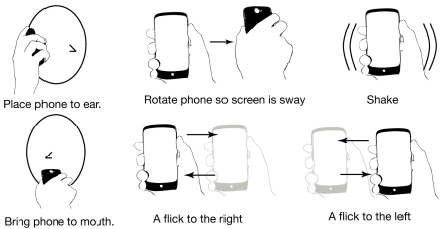
\includegraphics[width=0.7\textwidth]{images/gestures.png}
        \caption{Potential actions for gesture input}
        \label{fig:Gesture}
\end{figure}

The majority of previous literature has focused on gestures as not being socially acceptable in particular locations or in the presence of a certain `audience' \citep{rico_usable_2010, freeman_rhythmic_2017}. The social acceptability of an interaction is generally assessed by asking a participant to carry out various tasks in different scenarios, or by asking them to imagine themselves performing an interaction in those scenarios. The participant's views are either recorded throughout the tasks \citep{ahlstrom_are_2014} or collected at the end using an interview \citep{rico_usable_2010}. Users can also be examined on various metrics to understand how well they carry out the gesture \citep{freeman_rhythmic_2017}. \citet{freeman_rhythmic_2017} detailed that mid-air gestures were very usable and completed easily when users were given instruction and found audio signals aligned well with their use due to the consistent eyes-free nature of the features. This provides ground for the opportunity that users will be able to get more used to and more easily gain the benefits of mid-air gestures. This will be explored with respect to the perceived social acceptance that is brought along with it.

Where gestures are performed was the focus of the study done by \citet{rico_usable_2010}. The author describes various types of gesture and explained why some of them are reasonable or should not be used. It is suggested that optimal gestures should mimic motions that people may come across in their everyday life as they can be more familiar. Gestures that are found not to be effective are of an emblematic style and have pre-existing meanings. These can therefore be confused for their already established connotations. The analysis was done to maintain and solidify that using familiar gestures will make it easier for users to become familiar with them, increasing their usefulness and therefore social acceptability.

Acceptance of an interaction method has also been found to have a strong correlation to where, with respect to their body, the user performs a gesture. \citet{ahlstrom_are_2014} found that if carrying out the gesture took more than 6~seconds, the user tends to not see it as acceptable, because it is more likely to attract attention. Gestures that require body movement more than a foot away from the body are also considered less acceptable. \citet{ahlstrom_are_2014} believe this to be purely for visual reasons as it may look unnatural to others and is more likely to attract unwanted attention. However, this could also indicate that users perceive an interaction technique to be socially unacceptable if they believe others around them will perceive them to be putting in an abnormal amount of effort to accomplish an interaction task. This was explored through this dissertation's research.

\subsection{Smart Glasses}

A wearable device is a broad term that covers devices such as Smart Glasses, Watches and Rings. Since these devices take the place of common fashion accessories, they have an inherent need to be socially acceptable. They must be aesthetically pleasing, up to date with current trends and comfortable, all while facing the same interaction challenges of other devices, systems, and applications. This study focuses only on the interactions with these types of devices, in particular Smart Glasses.

Research carried out by \citet{chuah_wearable_2016} attempts to understand the factors that determine the widespread adoption of smartwatches by the population. It was concluded that visibility and perceived usefulness are large factors in this adoption. This was explored to establish if it is due to the user wanting to appear visible and not using effort by others which makes them confident in using the devices --- and similarly other novel interaction techniques --- in social situations. Studies focused on the appearance of smart glasses \citep{chuah_wearable_2016}. It is found that a device and its interaction modalities being unobtrusive enhances its social acceptance. This was investigated to understand if this is common for other interaction techniques. It was decided if, over time, users will better understand interaction techniques to become more comfortable using them due to a new-found familiarity, even if they are slightly obtrusive.

The focus of this area of study was directed towards the social acceptability and the use fullness of the Snapchat Spectacles as the product was available to me, these are shown in \autoref{fig:Spectacles}. The purpose of this product and its interaction methods have been speculated in the technical community \citep{constine_why_2017}. It is often deemed that the product was a failure and never took off. It seems that even when people bought the device, they rarely used it consistently and often stopped using it after as little as one week \citep{constine_why_2017}. At the time of writing, there have been 3 iterations of the Spectacles and none of them have been close to being a common household item. The consensus is that the fear brought about by other data glasses \citep{koelle_dont_2015} hindered the Snapchat Spectacles prospects of achieving success.

\begin{figure}[h!]
    \centering
    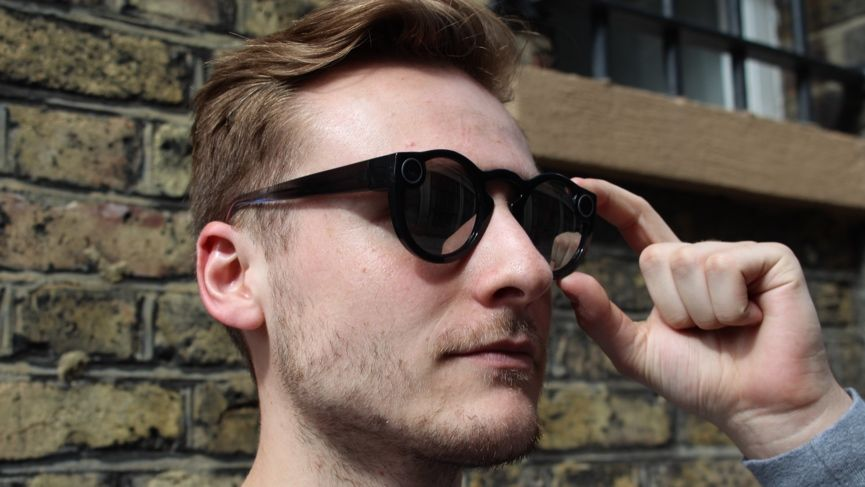
\includegraphics[width=0.75\textwidth]{images/spectacles.jpg}
        \caption{Snapchat Spectacles}
        \label{fig:Spectacles}
\end{figure}

\section{Effort, Usefulness and Acceptability}

There is a relationship between perceived usefulness and required effort in everyday tasks; when solving an immediate problem, a person will view it in comparison to their background of probable future problems \citep{zipf_human_2016}.  If a person sees an outcome as having less worth than the effort required to conduct the required task, it is likely they will not see it as a useful thing to do and will not want to do it. \citet{zipf_human_2016} also suggested that it is the social norm that a person will strive to expend the least amount of energy to solve a problem and accomplish a goal.

When interaction is viewed through this lens, if the input action to a device requires more energy than the desired output is worth, a user will not want to do it. Other literature strongly backs up this case in the context of personal user acceptance \citep{davis_perceived_1989}. \citet{zipf_human_2016} also believes that ``A person is socially treated according to the social signals he emits''. This, together with social norms of least effort, infers that one may not only want to reduce the effort to conserve energy but also, so it does not appear to others that they are wasting it. This may mean they would get treated differently. This study investigated if a reduction of energy consumption is purely for personal gain or if social pressures also have a part to play. 

A study of attitudes among students gave similar insight into the relationship between perceived effort, usefulness, and acceptance \citep{warrington_student_2000}. If one wants to be accepted by society, they must give off the correct norm of socially signals accordingly. In this study, it was found that from a young age, we learn that the social norm is to put in the least viable amount of effort to accomplish a task. This dissertation explored that if the acceptance of technology is governed by similar `rules'. Social signals coming from the effort expelled when providing input through novel interaction techniques was explored to understand if this is common among these circumstances. It may be socially desirable to minimise the amount of effort expended to accomplish an interaction task to avoid being seen to be trying too hard.

These implications were investigated in the context of novel interaction techniques, with a particular focus on how their perceived usefulness and social implications vary over time. It was hypothesised that the more a person uses a new interaction method, the more they will become used to using it and feel as though the desired outcome requires less effort. Therefor becoming more useful to them for accomplishing a task. Additionally, they may come across more useful functions as time passes that were not evident before use, increasing the value they will get by using it (potentially meaning it is acceptable to use more effort). These together will imply that a user will perceive the task to become more useful over time and less effort in comparison will be expended, making it more socially acceptable to do. 

Acceptance growing over time is examined in detail by \citet{hosokawa_walkman_1984}. The study detailed how over time, as people use or do something, it will gradually become more normal to them, it is referred to as ``The Walkman Effect''. Initial attitudes towards the Walkman were largely negative as it was a very out of the ordinary thing to use or be seen using in public. However, over time people became more familiar with it. Its clear function, usefulness, and ease of use lead to people being much more accepting of it. Before long, devices like this became the norm. This effect was investigated to understand if the same may also be true for novel interaction techniques, which have yet to achieve widespread adoption.

\section{Summary}

Various attributes have been linked to the social acceptability of novel interaction techniques through an array of studies. Common attributes consist of interaction being carried out in specific circumstances that are deemed unacceptable and how noticeable the integration is to others around the user. There have been few links made to effort required or usefulness. Social norms of least effort have been widely documented for general social situations. These social norms of least effort were further explored. A preliminary study was carried out to gain an insight into people's current perceptions of these links between effort and social acceptability and which novel interaction technique they may apply to most adequately.

%==================================================================================================================================
\chapter{Preliminary Survey Study}

\section{Introduction}

A preliminary survey was conducted to investigate perceptions of novel interaction methods. The aims of this survey were to begin studying perceptions of perceived effort and social acceptability, and to inform the design of a later experiment. At this early stage of the project, there were three ideas for the main experiment:

\begin{description}
    \item[Smart-glasses] The potential for an evaluation of the participants' usage and views of the Snapchat Spectacle wearable was considered. As this did not involve a substantial amount of technical development could be done easily in conjunction with another method. This evaluation could collect data from different participants, detailing their frequency of use, opinion of usefulness and acceptability levels over some time.  

    \item[Speech] The opportunities for developing an application for either the Amazon Echo or Google Nest were investigated as both devices were available to me and have been widely adopted in recent years. A potential study would explore how participants' use the device. For example, did they attempt to use speech all the time, or did they simply control the speaker within the assistant and other devices using their mobile device as a remote? 

    \item[Gestures] Another possible option for the experiment was to develop a mobile app that made use of a gesture interface. These could be touch gestures, mid-air gestures or device motion gestures. The experiment could cover usage and opinions of the features and interaction style, also looking into ease of use, usefulness, and social acceptability.
\end{description}

The survey, therefore, aimed to explore perceptions surrounding these interaction methods, to inform the main evaluation in this project. It gathered data about familiarity, prior experience, and preference of using these interaction modalities, as this would likely have an impact on perceptions of usefulness and acceptability.

\section{Methodology}

A survey was created and distributed to a sample of 24 participants, varying in age, gender, and technical knowledge. Participants were briefed on the aims of the research as a whole, as well as the aims of the specific questionnaire. Consent was granted by all participants and they were informed that they may withdraw from the process at any time, they were directed to the relevant people had they had any questions throughout, as per the ethics checklist. 

At the start, participants were asked to detail their views on how the amount of effort a task takes affects their likelihood to complete it (in general, rather than specifically related to interaction). They were asked to elaborate on if they had ever avoided putting effort into a task for social reasons and if they were aware of a social slur surrounding this issue of avoiding applying excess effort to a task.

Following this, participants were asked to gauge on a Likert scale how socially acceptable using certain novel interactions in a specific location may be. This was then also asked for the case of the same task outcome and situation but simply using the touch screen alternative method on their mobile device, as opposed to the novel interaction technique. They were asked about the relative effort compared in the two circumstances. They were asked to detail if they frequently use any of the range of interaction techniques and given the opportunity, in what circumstances they would happily use them and perceive it to be socially acceptable.

Finally, participants were asked to recommend what Gestures they would see fit for various functions that do not currently have associated with gestures in common devices. These were targeted to the functions that could be used in an app that could be created with integrated gesture input potential.

The preliminary study survey can be found at \autoref{appendix:questionnaires}.1

\section{Results and Reflections}
Participant responses to the survey questions were transferred to an Excel Spreadsheet, removing erroneous or incomplete data in the process. Analysis of responses is presented in the following sections, structured by theme.

\subsection{Social norms related to perceived effort}

Half of the participants would not see it as appealing to undertake a task which required more effort than the output. An additional third thought that others, be it colleagues or fellow students or sports team members etc, would look at them badly for putting in this effort, detailed in \autoref{fig:reward}. This reinforces the idea that people believe there to be a social norm that you should avoid putting in extra effort when you do not need to, as discussed in Section 2. 

\begin{figure}[h!]
    \centering
    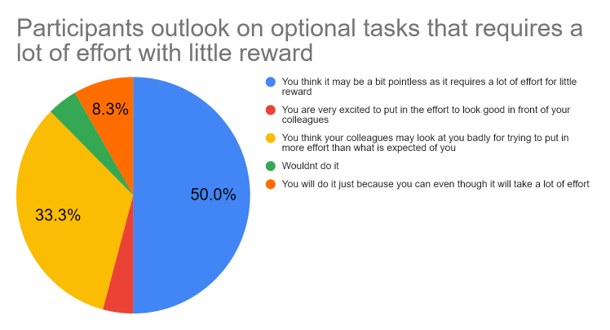
\includegraphics[width=\textwidth]{images/littleReward.png}
        \caption{Details of participants' responses to the question "You are given an optional task that requires a lot of effort (e.g. an optional exercise at college/University or an optional unpaid training session at work). Select from the following which best describes how you would feel about it?". Optional responses are detailed in the legend.}
        \label{fig:reward}
\end{figure}

Only four of the participants said that they had never avoided appearing as though they had put in more effort into a task than what was required. Many of the participants gave examples of when they do this, some included hiding how much you study for tests, how hard they tried to get a job so as not to appear like they needed to put in extra work in case others think they are struggling. Building on the idea that people do not want to appear as though they are trying harder than necessary to complete a task. The results also introduce the idea that people do not want to look like they must practice too much and put in too much effort to get good at something. People want to make it look like what they are doing has been done easily. 

The participants were presented with a mildly insulting name someone may call another if they feel as though they are going over and above what is expected of them. Every single participant knew its connotations and were able to explain that they were negative. People are very aware of the norms of "trying too hard" to do something and the repercussions of doing so. Many people are sucked into this way of thinking and it has become accepted that one must not appear to be trying too hard to achieve something, be it their life goals or a small daily task.

\subsection{Perceptions of acceptability of novel interaction methods}

There seemed to be some confusion understanding questions related to technologies that participants were aware of and those that they use at least weekly. Some participants said that they used some technologies on a weekly basis yet did not say that they were aware of them. This did not seem to make sense so following the closure of the survey, participants were asked some additional questions about the survey. They were asked to detail their understanding of this question. It was noted that some participants thought that the questions meant they were to select what technologies they were only aware of and had never used. It can therefore inherently be assumed that where a participant uses a technology, they also are aware of it. With these adjustments, all participants stated they were aware of Voice assistants with 70.8\% using them on a weekly basis. Half of the participants were aware of Gestures with only a quarter claiming to use gestures on a weekly basis. All but 2 participants were aware of what Virtual reality was, but yet only 2 claiming to use it on a weekly basis. A total of 54.2\% of participants were aware of the Snapchat Spectacles, again with only 2 claiming to use them on a weekly basis. No participant was unaware of any of these technologies, but 6 participants did say that they did not use any of them weekly. This can be easily visualised in \autoref{fig:familiar}.

\begin{figure}[h!]
    \centering
    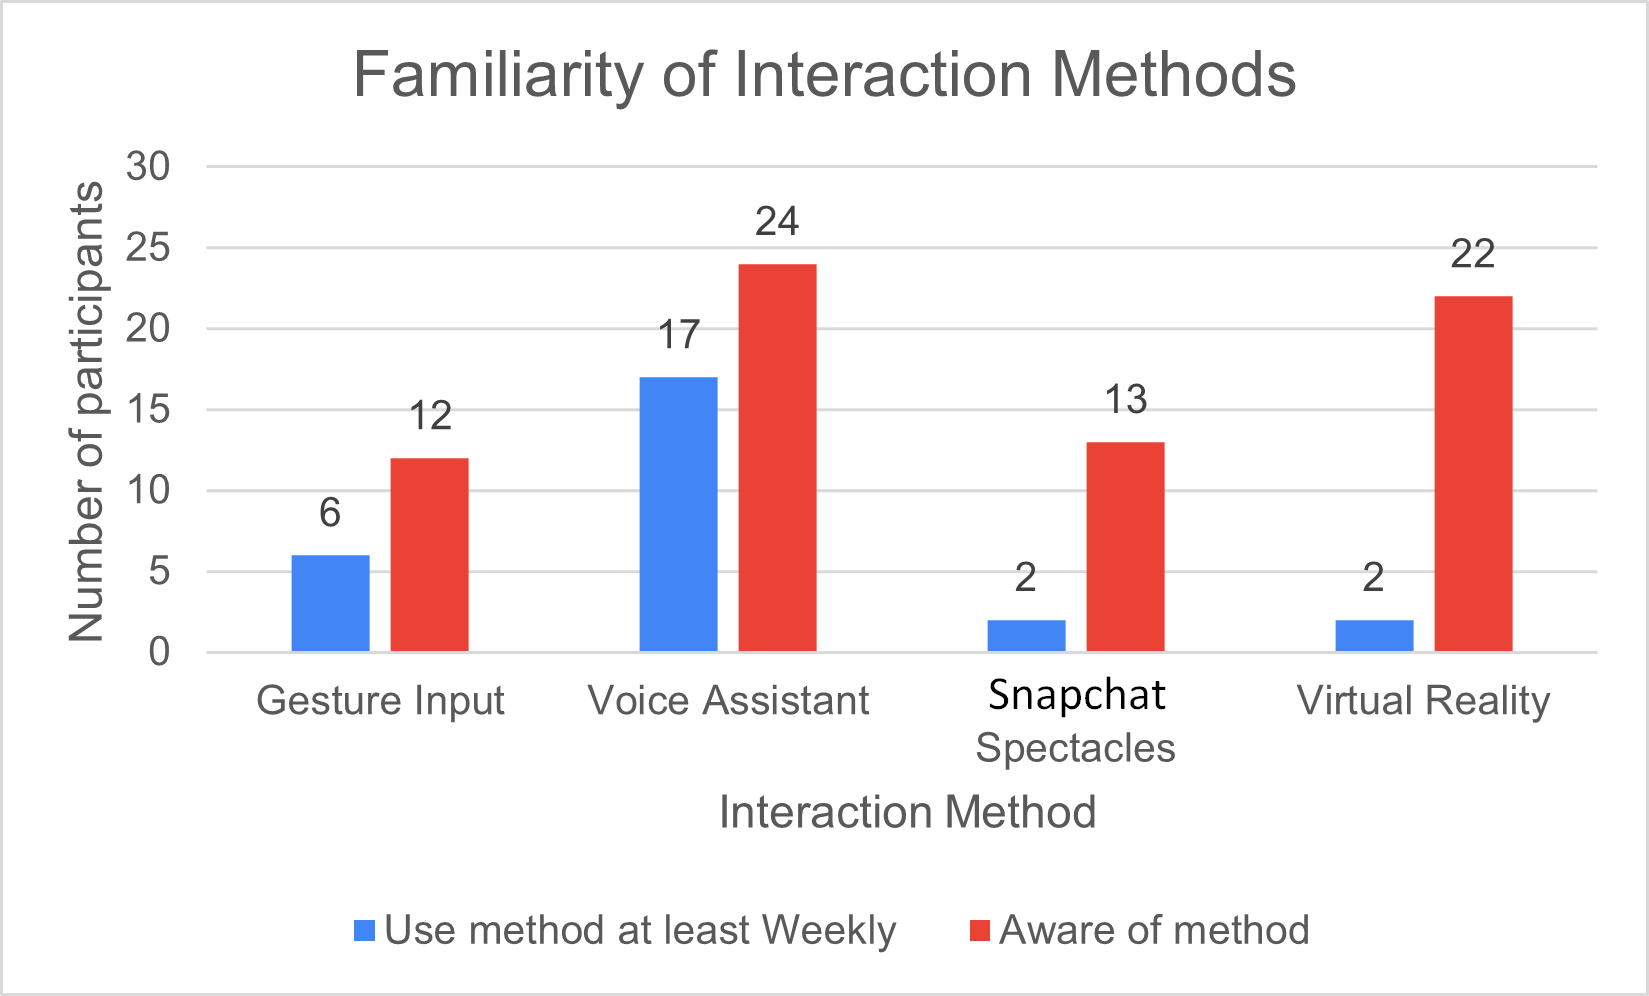
\includegraphics[width=0.9\textwidth]{images/familiarity.png}
        \caption{Bar chart detailing how many participants were aware of each interaction method presented to them and which of them they used at least weekly.}
        \label{fig:familiar}
\end{figure}

For questions relating to how participants perceive using a shuffle feature on a mobile device, a total of 91.67\% of people rated using a mobile phone's touch screen interface a five out of five for acceptability with the remaining, participants' rating it a four. Suggesting people are very familiar with using a touch screen interface and see no reason why it would be unacceptable to use. The average acceptability rating of using a device motion gesture was 4.25, slightly less than the touch screen alternative rating of 4.92. This is not a substantial difference yet does still infer that there is less confidence around using gestures. When determining what participants believe to use more effort there was a 45.8\% to 54.2\% split. This may infer that participants have a very varying opinion of the use of touch screen versus motion gesture. This could be down to participants’ unfamiliarity with the technology as 75\% of participants claimed that they do not use them on a weekly basis. It was stated that the most common reasons for a person not to use a gesture was if they were unhelpful (70.8\%) or not easy to use (66.7\%). Less than 17\% believed that ``company'' would affect this and only an eighth of participants thought their location would change their mind not to use gestures. This was considerably less than the other interaction methods.

When asked about their perceptions of taking pictures and short videos when on a walk with friends, the average rating of how acceptable it is to take a picture with your phone was 4.58 on a five-point scale, determining participants find this very acceptable. On the other hand, participants gave wearing and using the wearable, Snapchat Spectacles, an average rating of less than 2. Inferring many people believe this to be particularly unacceptable. Over 70\% of participants were under the impression that wearing the Spectacles would be more effort than simply taking your phone out and taking a picture with that. This could very well be the reason for people finding this method unacceptable. Participants’ reasons to decide not to use spectacles backs this up. A total of 75\% of participants felt that the technology not being useful and taking a lot of effort with respect to the desired outcome would change their mind about using the technology. Again, falling in line with two thirds of participants believing it not being easy to use being a strong reason to avoid using the technology. Less than 30\% said that using the spectacles in an unfamiliar company would make them rethink its use and only a quarter felt that they would be affected by the location. 

Questioning participants about setting a timer produced the following responses. Setting an alarm on a mobile phone using the devices touch screen received a high average acceptability rating of 4.79 of 5 from the participants. Doing the same task using a voice assistant received a moderate average rating of 3.54 of 5. There was a further agreement with participants in that using the voice assistant takes more effort, with only just over a third believing it is easier to use the voice assistant. This correlates well with the individual ratings as they seem to be very segregated. A third of participants rated the voice assistant a 5 for acceptability, a single parson rated it 2 and the remainder rated it a 3 out of 5. In general, where participants rated Voice assistants 2 or 3 they said it would take more effort to use than the phone and conversely for participants giving it a rating of 5. This had very little variation suggesting there is a very divided view of Voice assistants. It was thought that this might be due to participants' familiarity of using VAs by either learning that they were not as easy to use as they appeared, as found in the study done by \citet{myers_patterns_2018} or by learning that they took little effort to use. Yet it was found that there did not seem to be a great correlation between these two attributes where the participants were familiar. However, there was only one person that was not familiar with the technology and thought it would take less effort. The other 6 that were unfamiliar with VAs thought it would take more effort than the mobile phone's touch screen alternative. Participant’s stated they would avoid the use of VAs due to it either being not useful or not easy to use --- just over half for both. However, the company the user is in did seem to affect the participant's opinions VAs as much than in other technologies.

\subsection{Participant Gesture preferences and suggestions}

Participants were provided with mobile device functions ordinarily controlled though touch screen or other hardware interaction. They were asked to provide an example of a gesture alternative that they felt would naturally fit that function. Responses were coded into 5 categories; (1)~ No Answer, (2)~ Touch Gesture, (3)~ Mid-Air Gesture, (4)~ Device Motion Gesture, and (5)~ Other. It must also be noted, during error correction, if a gesture was out of the reasonable technical scope or did not include a gesture, no answer was noted unless any additional opinion was stated.

Participants were given the hypothetical task of adjusting the volume. Instead of pressing the volume up button, 8 participants opted for a touch gesture, 6 for mid-air and 5 for device motion. 5 participants gave no response. Instead of pressing the volume down button, 7 participants opted for touch gesture, 7 for mid-air and 5 for device motion. 5 participants gave no response, one provided an alternative option. To adjust the volume people preferred touch and Mid-air gestures over device motion gestures. This is likely caused by the more controllable nature of these interaction types over definitive intervals. This would suit the nature of volume adjustment.

When presented with the opportunity to skip to the next song playing on the device, 6 participants did not provide and answer. 8 provided a touch-based solution, 5 provided a mid-air gesture, 4 opted for a device motion gesture and a single participant responded with a solution that was considered Other. Most answers were reverting to various touch options, suggesting that the participants were failing to think of more innovative ideas of what gestures could represent this task. The number of answers for mid-air and motion gestures were both low with mid-air gestures having a slight edge in preference.

Participants were tasked with stating an alternative method of pausing and playing music. 7 participants supplied a response under the No Answer category and 2 under Other. 8 recommended a Touch gesture with only three favouring both mid-air and device motion style gestures. The number of participants that did not give an answer of a gesture increased. This suggests that the participants were running out of creative ideas to answer with, most answers reverting to various touch options, again reiterating that the participants losing interest. The number of answers were again low for mid-air and motion gestures.

Overall, there is a lack of results of device motion gestures. It is thought that the results are biased against this due to many people being unfamiliar with the use of gestures. In general device motion gestures are infrequently used within current technology so many of the participants may not be familiar with its potential and therefor failed to give an answer including it. Answers that did include device motion gestures tended to be more in detail which also suggests that it may be participants that are more familiar with the capabilities that suggested them.

\section{Discussion}

Participants seemed aware of the social norms of least effort. This supports the reasoning for exploring how these social norms may come into play when considering the social acceptability of novel interaction techniques.

It was decided that the focus of this research project would be mid-air and device motion gestures. Many factors were considered when making this decision. Voice assistant interactions were found to already be commonly used among the participants with many already being familiar with their use and having already formed strong opinions about their utility and acceptance. Experimentation with Snapchat Spectacles would not be reliable. Only one device was available and to ensure a reliable sample size, users would not be able to use them for a sufficient time to become familiar with them to detect a substantial change in opinion and vice versa. There seemed to be no resolution for this trade-off. This method would also lack external validity as claims could only be made about this specific device due to its individuality. Gestures were found to be the most practical and safe option during the Covid-19 pandemic. Users were able to download an Android app that implemented mid-air and device motion gestures without the need for any physical meeting or exchange of a device. 

Users appeared to understand these types of interactions without having experience using them. This enabled the potential for participants to increase their current use of the interaction technique and therefore introduce the ease of use and usefulness that will be found. These attributes effects on social acceptability were measured over time. This lack of prior knowledge of these gesture types was shown in participants' responses in the survey, they were unable to consistently provide reasonable gestures that were used. 

Inspiration for the gestures that were implemented was taken from survey responses and guidelines from other appropriate literature \citep{rico_usable_2010}. Gestures were designed to be familiar to users through being similar motions to other tasks yet without being emblematic of hand signals that may already have social meanings and are used in society. A shake style device motion gesture was developed to initiate playing a random song in a media player. This was inspired by the shaking motion one may make before rolling dice, the result of each being a random outcome. It was possible to pause or play a song by holding a hand in front if the device, taking inspiration from both user responses and the stop sign one may use (e.g. a police officer stopping a vehicle). These share the common trait on directing something stop, while unlikely to be confused for one another.

%==================================================================================================================================

\chapter{Technical Development}

Android was chosen as a development platform to enable the experiment to take place remotely using a user's own device. Based on earlier work in the project, mid-air gestures and device motion gestures were chosen as two novel input modalities for the User Study. An Android application enabled users to interact using these methods. The widespread adoption of Android mobile devices made evaluation participants easily accessible. Remote usage was important due to the COVID-19 restrictions. Since the intended use of the app was for a longitudinal evaluation, the app needed to provide functionality that people were likely to use frequently. For this reason, the app that was created was based on a music player application. Many people use these types of apps frequently and are familiar with the functions available. 

The following details the process in which the required application was developed. It notes the decisions made, particularly when issues were encountered, as well as the testing that was carried out and the reasoning for it. The application would be named Motion Music.


\section{User Interface}

\subsection{Design}
Ensuring that the base app was usable was essential in this development. It was vital that no part of the app was unusable or caused problems for the user, which could have an unwanted impact on user perception of the interaction techniques. Information collected about users’ opinions over time was focused on the gestures and other interactions, not other aspects of the user interface. Paper wireframes were initially drawn followed by a digital prototype. Figma desktop app was used for this as there was a free student version available with no time restriction. It was found to be an advanced system with a very realistic end-product, leading to quality prototypes.

Simple low fidelity paper wire-frames were created. Examples of such are shown in \autoref{fig:paperWF}. These were used to gain an understanding of what the app could look like and how users might want to use it. Initially, there was a home page with three destinations: (1)~Tunes, (2)~Artists and, (3)~Information. The Tunes page would show a list of all songs available. The Artist page would show a list of all artists, which would then lead to a further page showing all songs by that artist. The information page described the purpose of the app and gave help text about how to use it. When a song was clicked via the song or artist page, this would start playback and open the player page. On this page there would be options to pause, play, skip forward or skip backwards. There would also be a seek bar that shows progress through the song. The user would also be able to go back to the song or artist page they first clicked a song on to view other songs.

\begin{figure}[h!]
    \centering
    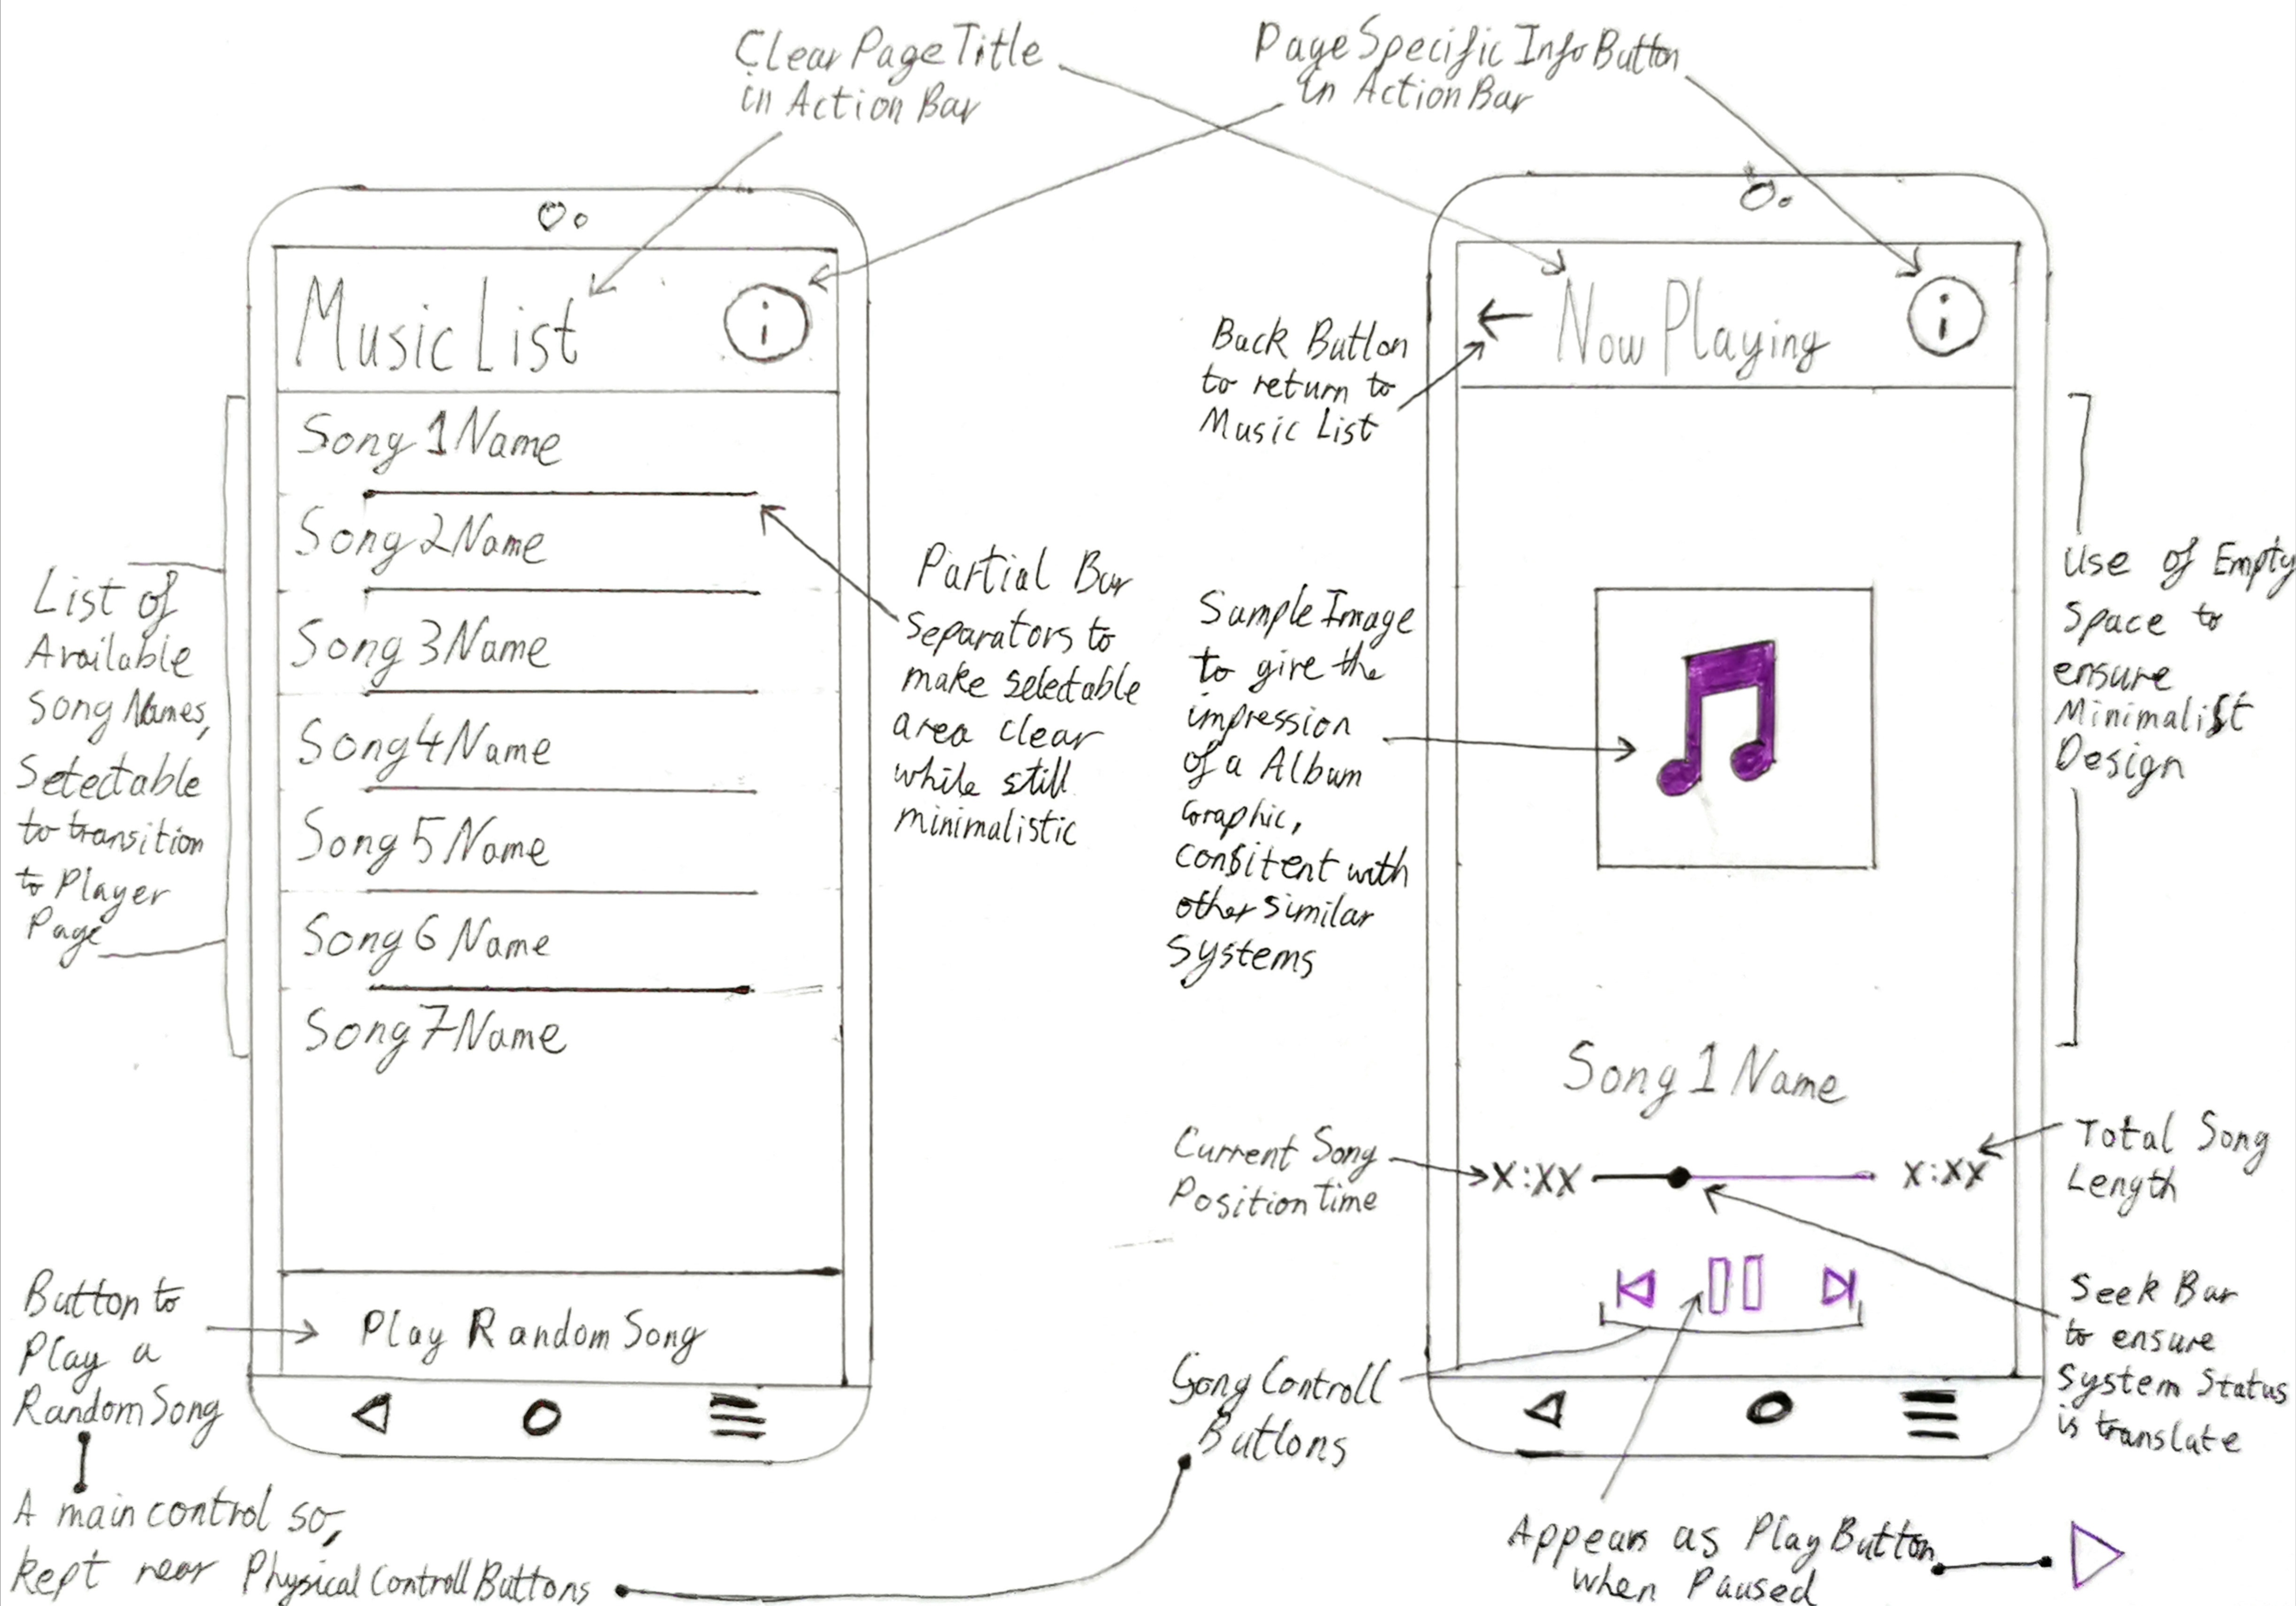
\includegraphics[scale=0.0675]{images/papWF.jpg}
        \caption{Paper wire-frames of the Song List and Player Pages, noting various design attributes and reasoning for them.}
        \label{fig:paperWF}
\end{figure}

A heuristic evaluation was used to identify improvements for the final wireframe prototypes, prior to implementation. Examples of the final wireframes are shown in \autoref{fig:digitalWF}. These wireframe designs were then adapted for implementation in Android. When adapting the design for the User Study, the app structure was simplified into a single page showing a list of songs. This decision was made to simplify interaction during the evaluation. Each page would have its own designated information page, accessible on the action bar, to provide assistance (e.g. for performing the mid-air gestures). A Random Song button was also added to the list page.

\begin{figure}[h!]
    \centering
    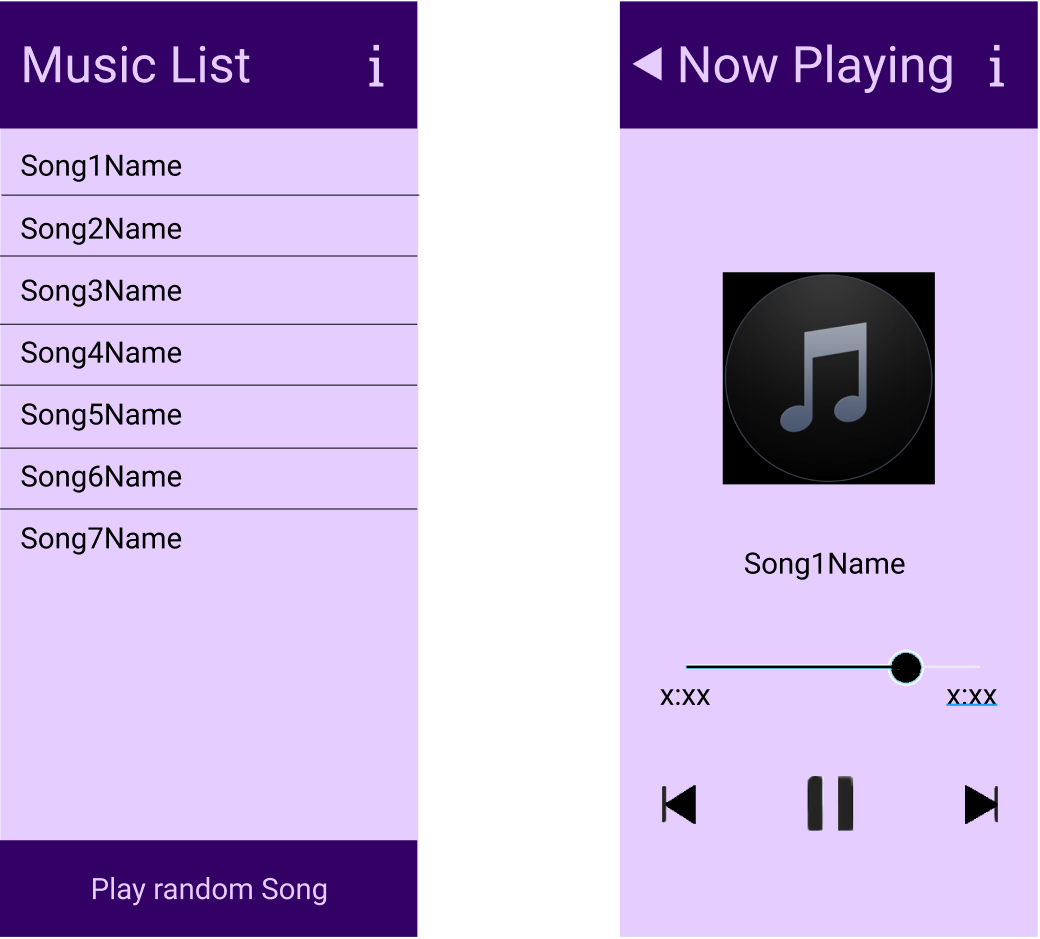
\includegraphics[width=0.75\textwidth]{images/DigWireframes.PNG}
        \caption{Digital wire-frames of the Song List and Player Pages, proving a detailed design and platform for exploring flow of the application}
        \label{fig:digitalWF}
\end{figure}

\subsection{Implementation}
An activity was first created to show a list of all .mp3 and .wav files on the device, the Tunes Activity. This was done by searching the device storage for files ending with .mp3 or .wav at the top file hierarchy of the device storage and then recursively check this for each subsequent child folder until storage has been checked. To do this it was required that the user granted permission to the application to access its storage --- This was also required to access the sensor data used to detect gestures. If this was not granted, then it was not done, and the user was informed of the consequences of this and directed to how permission can be changed to be granted.

Following this, a second activity was created to be the Player page. When any song on the list on the Tunes activity was selected, this initiated the Player activity and began playing that song. Buttons were created on this page to allow the user to pause the music if it was playing and play it again if it had been paused. These buttons were placed in the same position with the intention of only making them visible and press-able when appropriate. For example, if the music was already paused, the pause button would not be shown and unable to be pressed. Buttons were also added to skip to the next song in the list and play the previous song in the list. If the current song was at the end of the list; it would loop back round to the first in the list if the next button was pressed. The same goes for if the prev button was pressed when the current song is first in the list. 

The file name was also shown on the list page. It was decided that the file type (.mp3 or .wav) would again be stripped from the end to make it more recognisable to the user. The text also moved across the page if it were too long to fit to ensure the user would be able to read the full name. The user had the option to go back to the Tunes activity using the back button in the action bar. Finally, a button to play a random song in the list was implemented to be fixed at the bottom of the Tunes view. This would generate a random number with a maximum equal to the number of songs available. The song in this position of the list would then be selected and it would begin playing. Information buttons were added to the action bar on each of the pages. This triggered a pop-up box, detailing what gestures were possible to do on each of the pages. Images were also shown on the popup to demonstrate how to perform the gesture. These could be exited by tapping anywhere outside the popup box.


\subsection{Challenges}
There was a seek bar to be implemented on the Player activity in an attempt to give users more control and for them to have a better understanding of system status. However, during testing, many issues were found when the song finished, the seek bar would not align with the position of the next song. Nor would it follow the position of the song after the node was moved by the user. There seemed to be no consistencies of when it worked correctly and when it did not. Much time was spent in an attempt to fix this, but the root cause could not be found. At this time, the decision was taken to remove this feature as it was not an integral feature of the system. Additionally, if not all bugs were found in it then it could become a distraction to the user, and they may lose confidence in the application and create bias and skewed results.

\section{Music Playback}

\subsection{Asset Sourcing}
Due to the nature of the application, music assets needed to be sourced as participants would need to be able to interact with a music library and control music playback. If participants did not have access to audio files on their smartphone (e.g. due to their preferred use of streaming platforms), they would be unable to interact with the app for evaluation. To counter this it was required that users were provided the option to easily download music files. The platform that was used for this was ccMixter operated by ArtisTech Media. This is a site that provides free-licensed audio samples for commercial and non-commercial use. It provides proper means of attributions and crediting for the purpose of the Creative Commons License which covers all audio files available on the site. This platform was one of many of a similar style that could have provided the appropriate platform. This one was chosen as it had various documentation detailing how to use correctly and legally, what the creators and contributors provide.

\subsection{Implementation}
Various methods to implement the audio playing feature were considered. The two that were focused upon were (1)~The Android MediaPlayer APIs or, (2)~The Spotify SDK. Android Media Player provided the possibility to play audio files from the user’s device files in the applications file system or from a data stream over a network. This gave flexibility of how the audio files would be provided to users while also remaining stand alone and non-reliant on other systems. Using the Spotify SDK would infer a reliance on the user having access to Spotify and depend on the Spotify application working correctly. This means there could be issues with different types of Spotify accounts, shared accounts and also narrow the potential participants as some people may not use Spotify. It would also infer that if for some reason a user's Spotify app were to fail then the Motion Music application would also cease to run smoothly, giving the participant a negative bias towards the app and skewing the results. For this reason, it was decided to use the Android MediaPlayer API. The aim was originally to embed the audio files within the application file system, but this was later changed to read files from the user’s device. This allowed users to listen to their pre-existing music already on their device and not have to use the music supplied. This was decided upon as it gave the user more freedom and customization, increasing the usability heuristics of the application and reducing external factors that may affect results gathered from participants.

\section{Mid-Air Gesture}

\subsection{Design}
A mid-air gesture was designed to control music playback, by toggling playback state:, pause the music if it was currently playing or start playing music again if it had previously been paused. This gesture would only be accessed when the Player activity was active. The command would be activated by conducting the gesture of holding a hand above the front of the device, around an inch away from it, as shown in \autoref{fig:Mid-air}. This gesture design was chosen at it may be familiar to the users since it is similar to a stop hand signal.

\begin{figure}
    \centering
    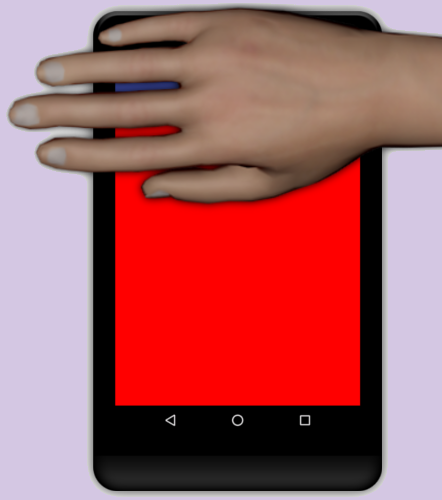
\includegraphics[width=0.6\textwidth]{images/covering.png}
        \caption{Graphic displaying how the mid-air gesture of covering the front of the device to play/pause music can be activated.}
        \label{fig:Mid-air}
\end{figure}

\subsection{Implementation}
This mid-air gesture was initially implemented by measuring the ambient light sensor on the mobile device: i.e. if it became substantially lower whilst the screen was unlocked, it was assumed a person's hand was being held over it. However, it was later found during testing that the light level in the location impacted the gesture success rate drastically. As an alternative, the proximity sensor was used instead. A threshold-based approach was used to detect when a gesture occurred. A baseline proximity reading was established during idle use. When the proximity value changed so that the current value was less than 80\% of the previous baseline, then the play/pause button would be activated, as shown in Algorithm \ref{lst:Proximity}. This threshold value was determined through informal pilot testing to ensure it was reliable. This gesture could not again be used again until the initial instance was complete and the hand was moved away.

\begin{lstlisting}[language=java, float, caption={Java code detailing how the Pause/Play gesture is detected and how it is acted upon.}, label=lst:Proximity]

proximity.setListener(new Proximity.Listener() {
    @Override
    public void onCover(float prox) {
        // Only compare if there is a previous value to compare to
        if (!firstProx) {
            // Check if gesture has been detected
            if (prox < lastProx * 0.8) {
                //Act on gesture detection
                pause.performClick();
                // Rnsure next iteration is missed
                firstProx = true;
            }
        // Determine if it is the first pass
        } else { firstProx = false; }
        lastProx = prox;
    }
});
\end{lstlisting}

\subsection{Challenges}

As previously stated, following the initial testing of the mid-air gesture, the detection was found to be unreliable. In this case, it was due to the nature of the light sensor. If there was very little ambient light in the room, the light level when no gesture was being completed was very low. The intention was that when a significant change occurred in the light level then it would be assumed that the gesture was being performed. However, this low level in the ambient state meant that when the gesture was being performed not a large enough change was being detected. However, this could not simply be amended by lowering the threshold of change that was required as other changes in light level were also affecting reliability. For example, if there was a light on in the room that was turned off, a significant change was detected, and the device interpreted this as the gesture being performed when this was not the case. It was decided that too many external factors were interfering with the light sensor. To counter these issues, the fix was to instead use the proximity sensor. Smartphone proximity sensors use infrared light so are more robust against ambient light variation. This would ensure external light levels would not affect performance. It was originally not used as it was thought the user may need to get too close to it but after it had been implemented in the same way as the other sensor detectors it was found to be very efficient.


\section{Device Motion Gesture}

\subsection{Design}
A device motion gesture was also implemented to control playback. The function of which was to begin playing a random song from the list. This gesture could be performed when either the Tunes or the Player activity was active. The gesture would be performed by simply shaking the device, as shown in \autoref{fig:Dev-Mot}. This was chosen as a suitable action as it mimicked the motion of rolling some dice to give a random number, in this case, a random song. The gesture would be accessible in all areas of the application, even when a song is already playing.

\begin{figure}[h!]
    \centering
    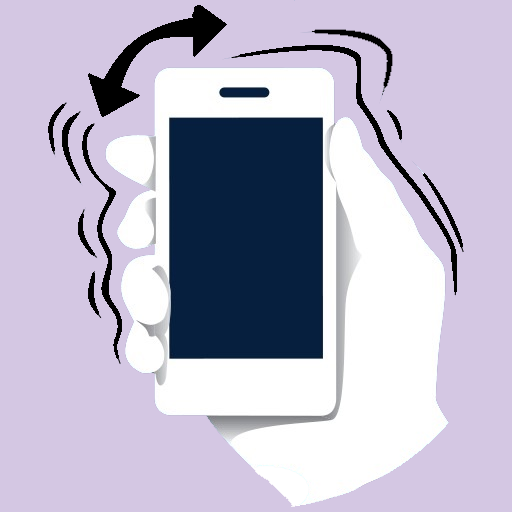
\includegraphics[width=0.575\textwidth]{images/shaking.png}
        \caption{Graphic displaying how the device motion gesture of shaking the device to play a random song can be activated.}
        \label{fig:Dev-Mot}
\end{figure}

\subsection{Implementation}
This gesture was implemented using the device accelerometer to detect sudden and substantial motion. If there was a notable increase in acceleration, then the music player would infer that this gesture was being performed. The accelerometer data stream was gathered again by making use of the SensorEvent values. The accelerometer would provide 3 values, the acceleration force along each of the x, y and z-axis. Following the previous gesture, the initial values of the sensor data were not checked to see if a gesture was detected to ensure errors were prevented. The first set of values would not have anything to be compared to. The gesture was detected in the difference between the current value and the previous value in at least 2 axes were found to be greater than a threshold value, as shown in Algorithm \ref{lst:Accelerometer}. Only 2 axes were required to exceed this threshold as it was found that when shaking a device, this often only results in substantial acceleration across one or two main axes, with the third typically remaining low. If all three were required to meet the threshold this would become very difficult for users to complete. Initially, a fixed threshold acceleration was chosen based on pilot testing with a personal device.

\vspace{15mm}

\begin{lstlisting}[language=java, caption={Java code detailing how the shake gesture is detected and how it is acted upon, this particular instance for when detection is made on the Tunes Activity.}, label=lst:Accelerometer]

accelerometer.setListener(new Accelerometer.Listener() {
    @Override
    public void onTranslation(float currX, float currY, float currZ) {
        // Ensure first pass is missed to ensure lastX, lastY and lastZ have values adn songs are available
        if(!accFirst && loaded) {
            xDiff = Math.abs(lastX - currX);
            yDiff = Math.abs(lastY - currY);
            zDiff = Math.abs(lastZ - currZ);
            // Calculate if change is higher that the htreshold in any two axis
            if ((xDiff > threshH && yDiff > threshH) || (xDiff > threshH && zDiff > threshH) || (yDiff > threshH && zDiff > threshH)){
                //act on gesture detection
                shuffle.performClick();
                accFirst = true;
            }
        // Dictate if it is the first pass
        }else {accFirst = false;}
        // Set the current values to be compared against n next iteration
        lastX = currX;
        lastY = currY;
        lastZ = currZ;
    }        
});
\end{lstlisting}

\vspace{15mm}

\subsection{Challenges}
A pilot test was done on various devices from various manufacturers with release dates ranging from 2016 to 2020. On various devices the shake gesture was too easily detected, requiring almost no motion at all, while others were unable to detect the gesture unless the device was very vigorously shaken. The reason for this is thought to be due to the sensitivity of the sensors used by different manufacturers. Devices from common manufacturers required the same vigour of shaking. This implied that a simple fixed threshold value could not be used, research was done to confirm this. 

To address this, a calibration step was required for the shake gesture. This was implemented by creating an activity that the user were met with upon opening the application for the first time. The user were directed to shake the device and then press a calibrate button. When the user shook the device, the accelerometer data was read, and a sample shake threshold was found by calculating the average of each of the highest values for each axis during the sample shake. This was used as a value to detect further shake gestures the user performed while using the main functionalities of the application, making it far more reliable across all devices. To ensure this calibration was controllable, an additional button was added to the action bar. This could be accessed by the user from anywhere on the application and returned them to the calibration step in the case that they had not performed the gesture in an ideal way on the previous calibration attempt. This button initiated a popup ensuring the user knew that this was what was about to happen. If they accepted, the user was successfully return to the calibration step. If it was not accepted by the user, the popup disappeared, and the current calibration was maintained allowing the user to continue using the application.

A similar pilot test was again run to ensure that this was a successful amendment to the system. However, some additional tests were done. To ensure the calibration worked successfully it required to only proceed if a reasonable shake was detected. To ensure this was the case the calibration was attempted without moving the device and checking if it allowed the user to proceed, which it did not. The shake required after calibration also needed to be of around the same vigour as was done in the calibration step. This was checked by calibrating with various levels of vigour and checking to ensure that this same level of vigour was what was required for the gesture to be detected.


\section{Testing}

Testing of the application was done in three general stages throughout the implementation. Android Studio provides the opportunity to run the application that has been created on an android mobile device emulator. This was used for the majority of the testing at the stage of creating and completing the music player user interface and its playback functions. Further testing was conducted using a single personal mobile device when implementing gesture detection. After the gestures had been initially implemented and tested on the single device, the application was tested over a variety of mobile devices to ensure working functionality for all potential users. Throughout the process, the debug function provided by Android Studio was utilised.

The first stage of coding development aimed to produce a music player application upon which the gesture capabilities would then be built upon. It needed to be confirmed that this portion of the application was fully functioning and without bugs or errors. As each component was added to the base activities, it was tested using the Android Virtual Device facilities in Android Studio. In this instance, a virtual Google Pixel 3a was used. This provided a means of running the application in a safe space without having to download and install it on a physical device. 


When viewing the audio files that were gathered from storage, files from other applications that were not conceptually intended for pleasurable music listening were included (e.g. ringtones and sound effects). This was countered by adding checks and restrictions to the names of the files that were being retrieved and made available. The shaking gesture was not detected so the constant threshold value was reduced to an appropriate value. Once this had been achieved, a random song started when viewing either the Tunes or Player Activities were active and shaking the device the appropriate amount, as expected. Edge cases were tested by moving the device in ways that would be presumed natural and ensuring that it was not registered as a gesture. As previously stated, the Light Detector that had been implemented at this point was found to be fundamentally flawed. Inferring the gesture unusable and other options were explored. This was found by moving the phone naturally through multiple environments and attempting the gesture in an attempt to find edge cases for registering the gesture. Music was successfully paused and played when the gesture was detected. This only happened when the Player Activity was active, as expected.


%==================================================================================================================================
\chapter{User Study}

\section{Outline}
The aims of this study were as follows. How participant perceptions of the effort required to use a gesture and how useful it is, change as time passes and they become more familiar with it. How this usefulness and ease of use relate to the perceived social acceptability will also be explored. Furthermore, it is hoped that attributes that affect how rapidly these changes occur will be found. Participants' views on where the future of gestures might lead to, and how they could be used practically, were also gathered and examined to better understand their true views on novel interaction techniques.

Participants' would experience using a novel interaction technique, that they had little familiarity with using previously. In this case, it was decided that the novel interaction technique in question would be device motion gestures and mid-air gestures. This technique would be made available to them on their personal mobile device. Ensuring the user is familiar with the environment in which the interaction technique is built is very important to ensure no other external factors on unfamiliarity infer secondary effect. Participants were provided with an information leaflet and consent forms to complete in line with the ethics checklist. Participants were then asked to complete surveys at a specific time frame during the experiment’s timeline. Collecting data throughout the experiment on the users' experiences is important to understand opinions as time passes. Results were processed and searched for erroneous input. Evidence of this was discarded from results. Statistical analysis was carried out using the Wilcoxon Rank Sum test and Results were analysed using other techniques. Results and their implications are discussed.


\section{Method}

\subsection{Recruitment}

Participants were required to have an Android device so they could run the Motion Music app. They were required to have limited experience using mid-air gestures and device motion gestures, to avoid influencing their perceptions of these interaction styles. Participants needed to cover a varying age range and technical knowledge to ensure that the sample is a proper representation of the population. Participants were recruited through social media and word of mouth.

Before any experimentation, participants were asked to read and complete a declaration of consent. An overall declaration of consent for this User Study was provided to participants electronically, detailing the aims of the overall research and individual requirements from the participants at each stage. It was made clear that a participant could ask for more information at any stage as well as ask to be removed at any time, in which case all data that was held relating to them would be deleted and not used in the study. Users were asked to provide further consent for every individual survey throughout the User Study. Each of which details the same as the above with additional details of the aims of that specific survey and how long they should expect to have to spend doing it. This would always ensure that the participants felt they had control over the data that they were supplying, while also being reminded where help can be found. When the final survey was completed by the participant and the study had come to an end, they were provided with an experiment debrief, containing information about what would be done with the data collected and how they could remain in communication in the case of any additional information they may require or if they wish to withdraw from the study.

\subsection{Procedure}

Upon commencing the research, each participant was supplied with an information leaflet. This again detailed the aims of the research along with the suspected timeline of the experiment and what would be required of the participant throughout. It provided information and instructions of how to prepare their device to run the application along with how to download and install the software required to take part. Information detailing hot to use the application and its potential use cases were described to ensure the participants were always well informed and understood what was required of them before agreeing to take part.

A pre-study survey asked the participant to say which type of gestures they believed their device to be able to recognise and how regularly they use each gesture type, if at all. They were asked to detail situations in which they would be happy to use one of these gestures if they had the option to use either the touch screen or the gesture for a required function. They were also asked to detail situations in which they would be happy to use one of these gestures if they had no option to use the touch screen for a required function. The purpose of this section of the study was to identify how much experience participants had with interaction techniques like these. It would also provide a baseline on their perceptions of gesture input, which could then be compared to their views during and after the week-long study period, to see if they had changed.

The pre-study  survey can be found at \autoref{appendix:questionnaires}.2


After completing this initial survey, participants were asked to install the Motion Music application on their device. Participants were also directed to download the music files sourced from ccMixter so the app had access to music for playback. This was not necessary if they had existing music files saved to their device storage or they could choose to download audio files from another source.

Once each participant had installed Motion Music, they were given instructions about how to use the application, what was expected throughout the week-long study, and when the following surveys should be completed. They were asked to refer to the usage guide in the information sheet for more information. This told them how to complete the calibration step when first opening the application, the functions it had, and the various ways of activating these functions --- through both the touch screen and the two types of gesture. This was done to ensure the participant understood the full potential of the application and were able to utilize all functions. It also meant that participants did not expect the application to do more than it was capable of, as this may lead to frustration which could bias results and their perceptions of the interactions.

Over the course of the User study, participants were required to complete 4 different surveys, all on different days. This introduced the issue of data continuity. Participants' responses to all the surveys needed to be coupled so that they could be compared over time. To do this, participants were asked to provide a pseudonym that would be provided at the start of all surveys to enable this to be done. To ensure anonymity participants were advised not to make this their name, email, username, password, birthday, address or similar that may relate to them. It was recommended that they use a random word, number, sequence, or other combination that they would be able to remember and supply throughout. Ensuring anonymity of these pseudonyms was of utmost importance to ensure that the participants were safe from any threats or dangers that could relate data back to them. Adhering to the intent of the ethics checklist was a priority. 

Following the pre-study survey, participants were asked to complete a survey after one day of use, after three days of use and after one week of use. These intervals were used to capture how users felt after briefly using the application, after using it for a short time and after a full week. Progress was tracked over this time to ensure surveys were distributed and completed on time. This was important to keep consistency as some participants started the process at different times. Each of the surveys aimed to track how much the participant used the application and what their perceptions and opinions of the gestures were. The three surveys asked the participant the same questions. The final survey had additional questions to allow the participant to reflect on the time they had used the application and gestures.

The survey for completion after one, three, and seven days of use can be found at \autoref{appendix:questionnaires}.3, \ref{appendix:questionnaires}.4 and \ref{appendix:questionnaires}.5 respectively

The three main surveys asked participants to detail their usage since the previous survey:
\begin{itemize}
    \item How many times they used Motion Music
    \item How many times they had used the mid-air gesture
    \item How many times they had used the device motion gesture
\end{itemize}

 This was to understand how frequently they were using the application between surveys. This would eventually be compared to see if it had an effect on how quickly the participants got used to using the application. 
 
 Likert scale questions ranging from strongly disagree to strongly agree were used to find user perceptions of:
 \begin{itemize}
    \item How useful each gesture was.
    \item How  easy each gesture was to use.
    \item How comfortable they would be using each gesture in an unfamiliar location or company.
    \item How gimmicky they felt gestures were in general - this was not asked per gesture to gain an insight to how users felt about the idea of gestures as opposed to the specific gestures
\end{itemize}

 The changes in users' perceptions between surveys would be explored. During each survey participants were asked: 
 \begin{itemize}
     \item To describe a time in which they thought that each gesture input type was more useful for a situation as opposed to simply using the touch screen input alternative.
     \item To detail some comments on the system as a whole, participants could supply their own response as well  as choosing to select one or more of the following: \begin{itemize}
         \item ``I found the gesture functions difficult to perform''
         \item ``I found it fairly hard to get in the way of using the gesture functions''
         \item ``I consciously went out my way to try the gesture functions''
         \item ``I tried to get better and more used to using the gesture functions''
         \item ``I found myself using the gesture functions without thinking about it''
     \end{itemize}
 \end{itemize}
These qualitative views were tracked and compared throughout the process.

Finally, the survey for completion after a week of use was completed by participants to investigate their experiences over the whole week. They were asked to indicate, across a variety of usage contexts, which of the gestures they felt was:
\begin{itemize}
    \item Easiest to use successfully.
    \item Most useful in this context.
    \item More socially acceptable.
\end{itemize}
Participants were also asked to rate, on a Likert scale, to what extent they Agree, or not: 
\begin{itemize}
  \item That they found themselves using the gestures without thinking about it.
  \item That they  found the week eye opening to the potential gesture could have.
  \item That they believe that mainstream applications don't currently and could make use of device motion and mid-air gestures
\end{itemize}
This was to be used to compare the participants' opinions on gesture use to what they previously thought about gestures before using the application. Participants were also asked if they had thought of a specific use gestures could have in other situations or by other applications.


\section{Results} 
8 people completed the week-long evaluation, 3 of whom were female and 5 male. 4 participants had prior technical knowledge and 4 had limited technical knowledge. The mean age was 30.4 years. This sample size was limited due to Covid-19 restrictions, which necessitated a remotely conducted experiment and made recruiting participants challenging. Participants were required to supply a uniquely identifiable keyword used throughout the evaluation, to track their survey responses over time and ensure the data from the three surveys were matched, while still ensuring anonymity throughout the results.

Survey responses were processed into a spreadsheet and prepared for analysis. For questions that asked participants to respond using a Likert scale, Strongly Agree was numerically encoded to a rating of 5, Agree to 4, Neutral to 3, Disagree to 2 and Strongly Disagree to 1. These values were then plotted upon line graphs. Data sets of Likert scale data between the various surveys were statistically analysed using the Wilcoxon rank-sum test to determine if there was a significant difference in participant responses between the surveys. This non-parametric test is appropriate because the data is ordinal and requires a comparison between two groups, i.e., two different time frames. A significance level of 5\% was used in the analysis. Themes in qualitative data were identified and patterns were found in order to draw conclusions.

\subsection{Usage Habits}

All participants use an Android phone as their personal device so were familiar with the operating system and interaction conventions used in the app. None of the participants believed their device gave them the option to use mid-air gestures for input. Half of them knew their device supported motion gestures and only 2 had previously used this interaction method; their reported use of this input modality was ``less than weekly''. If provided the option to use mid-air or motion gestures, a quarter said they would continue to just use the touch screen option, with remaining participants indicating that their preference for input would depend on whether the interaction would require less effort than simply using the touch screen. Additionally, one respondent said it would also depend on the social situation. Respondents who said they would continue to use the touch screen had indicated previously that they knew their device supported motion gestures but did not use them. When asked what they would do if a function required the use of motion or mid-air gestures, with no touch screen alternative:\begin{itemize}
    \item Two said they would ``never'' use that function
    \item Two said they would use it ``no matter what'', simply because they wanted to use the function
    \item One said they would use it ``if it suited the situation''
    \item One said they would use it ``if it was useful''
    \item One said they would use it ``if it took little effort to use''
    \item One said they would use it ``if it fitted the social situation but only if it was useful''
\end{itemize}

After one day of the evaluation only one person used the app up to 10 times. Remaining participants reported using the app up to four times, two of which only used the application once. 

After three days of use, apart from two people who used the app up to 10 times, participants reported using the app up to four times, with all participants using it at least 2 times. 

After one week, half the participants used the app a further 5-10 times and the other half said they used it more than 10 times. Usage frequency is shown in \autoref{fig:usage}.

Users tended to use the motion gesture equal to, or less than, the number of times they used the app while using the mid-air gesture equal to or more than the number of times they used the app.

\begin{figure}[h!]
    \centering
    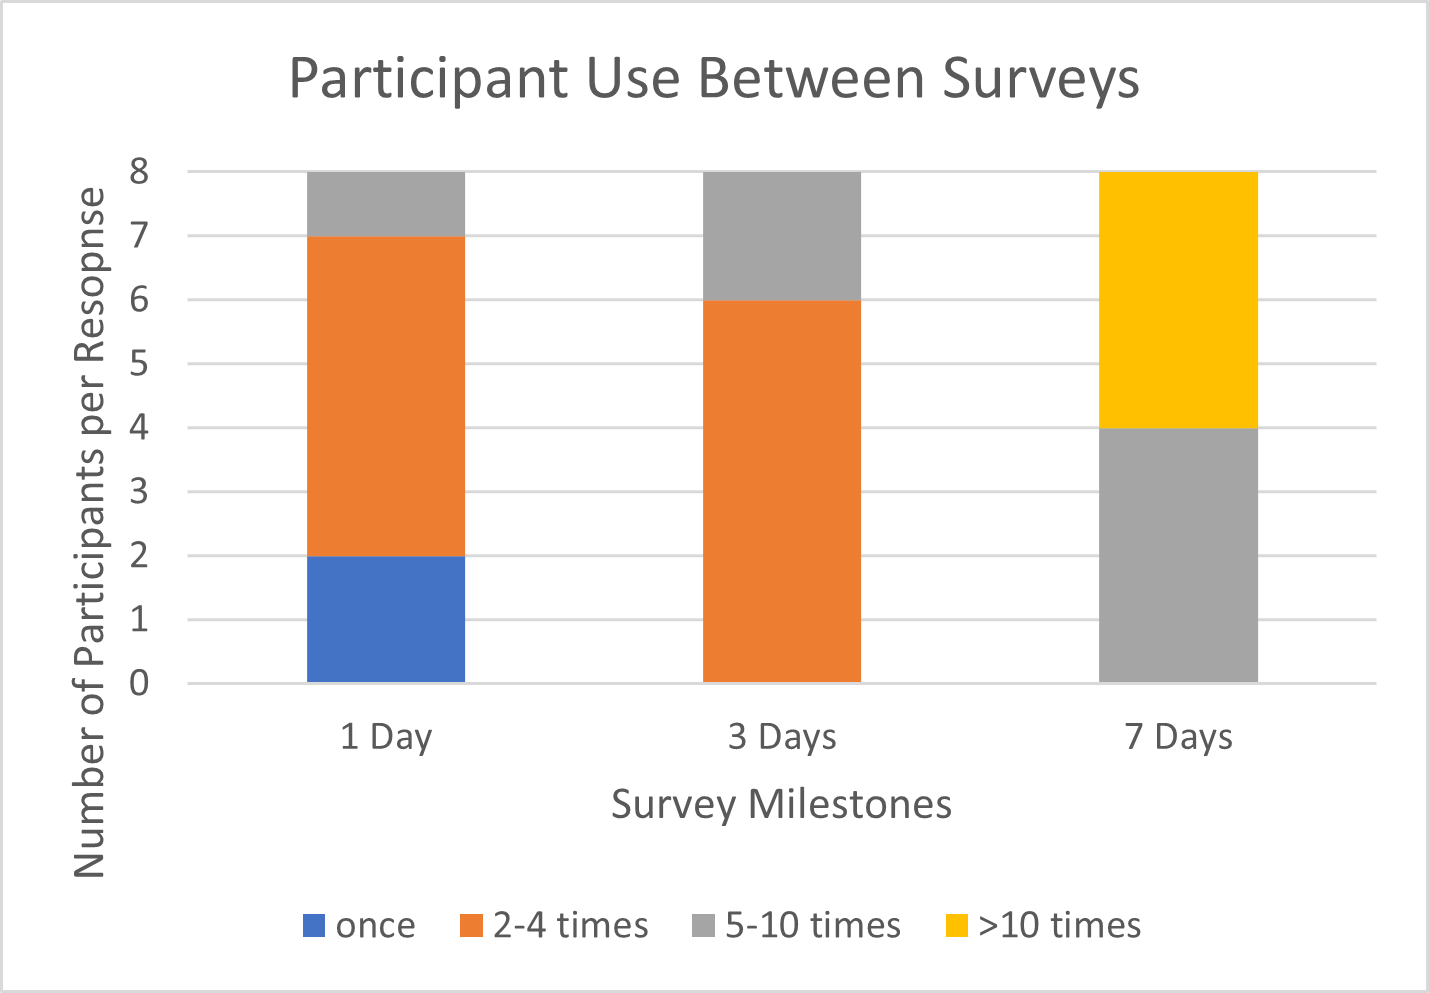
\includegraphics[width=\textwidth]{images/Stacked Use.png}
        \caption{Stacked bar chart showing the participants' usage of the Motion Music application over one week.}
        \label{fig:usage}
\end{figure}

\subsection{Perceived Usefulness, Usability and Acceptability}

\subsubsection{Perceived Usefulness}

\autoref{table:usefulness} shows mean responses to the survey questions about the perceived usefulness of the motion gestures and mid-air gestures. Ratings were on a five-point scale, where 1 was ``not useful'' and 5 was ``very useful''. Changes in how useful the participants felt the gestures are visualised on \autoref{fig:perceptions}. 

\begin{table}[h!]
\centering
\begin{tabular}{r c c c}
                              & \textbf{Day 1} & \textbf{Day 3} & \textbf{Day 7} \\ \toprule
    \textbf{Motion Gestures}  & Mean: 2.25, SD: 0.71   & Mean: 3.13, SD: 0.83    & Mean: 3.98, SD: 0.71  \\
    \textbf{Mid-Air Gestures} & Mean: 2.25, SD: 1.16   & Mean: 4.25, SD: 0.83    & Mean: 4.38, SD: 0.52 \\ \bottomrule
\end{tabular}
\caption{Mean perceived usefulness ratings and Standard Deviation.}
\label{table:usefulness}
\end{table}

Wilcoxon tests were used for pairwise comparisons between responses on subsequent days.

For motion gestures, ratings were significantly higher on Day~3 than Day~1 (p = 0.019, z = 2.33) and on Day~7 than Day~3 (p = 0.024, z = 2.26).

For mid-air gestures, ratings were significantly higher on Day~3 than Day~1 (p = 0.016, z = 2.39) and on Day~7 than Day~3 (p = 0.102, z = 1.63).
\hfill \break






\subsubsection{Ease of Use}

\autoref{table:Ease} shows mean responses to the survey questions about the perceived ease of use of the motion gestures and mid-air gestures. Ratings were on a five-point scale, where 1 was ``not easy to use'' and 5 was ``very easy to use''. Changes in how easy to use the participants felt the gestures are visualised on \autoref{fig:perceptions}. 

\begin{table}[h!]
\centering
\begin{tabular}{r c c c}
                              & \textbf{Day 1} & \textbf{Day 3} & \textbf{Day 7} \\ \toprule
    \textbf{Motion Gestures}  & Mean: 2.13, SD: 0.99    & Mean: 3.88, SD: 0.83    & Mean: 4.5, SD: 0.53\\
    \textbf{Mid-Air Gestures} & Mean: 2.38, SD: 0.74   & Mean: 4, SD: 0.76    & Mean: 4.88, SD: 0.35 \\ \bottomrule
\end{tabular}
\caption{Mean perceived ease of use ratings and Standard Deviation.}
\label{table:Ease}
\end{table}
Wilcoxon tests were used for pairwise comparisons between responses on subsequent days.

For motion gestures, ratings were significantly higher on Day~3 than Day~1 (p = 0.008, z = 2.64) and on Day~7 than Day~3 (p = 0.025, z = 2.24).

For mid-air gestures, ratings were significantly higher on Day~3 than Day~1 (p = 0.011, z = 2.53) and on Day~7 than Day~3 (p = 0.019, z = 2.33).
\hfill \break






\subsubsection{Social Acceptability}

\autoref{table:SocailA} shows mean responses to the survey questions about the perceived social acceptability of the motion gestures and mid-air gestures. Ratings were on a five-point scale, where 1 was ``not socially acceptable'' and 5 was ``very socially acceptable''. Changes in participants' confidence in using these gestures in unfamiliar locations or company are visualised on \autoref{fig:perceptions}. 

\begin{table}[h!]
\centering
\begin{tabular}{r c c c}
                              & \textbf{Day 1} & \textbf{Day 3} & \textbf{Day 7} \\ \toprule
    \textbf{Motion Gestures}  & Mean: 2.5, SD: 0.76   & Mean: 3.5, SD: 0.54    & Mean: 4.38, SD: 0.52  \\
    \textbf{Mid-Air Gestures} & Mean: 2.75, SD: 0.89   & Mean: 4.25, SD: 0.76    & Mean: 4.38, SD: 0 \\ \bottomrule
\end{tabular}
\caption{Mean perceived social acceptability ratings and Standard Deviation.}
\label{table:SocailA}
\end{table}

Wilcoxon tests were used for pairwise comparisons between responses on subsequent days.

For motion gestures, ratings were significantly higher on Day~3 than Day~1 (p = 0.039, z = 2.06) and on Day~7 than Day~3 (p = 0.019, z = 2.33).

For mid-air gestures, ratings were significantly higher on Day~3 than Day~1 (p = 0.014, z = 2.46) and on Day~7 than Day~3 (p = 0.023, z = 2.27).

\hfill \break






\subsubsection{Gimmicky}

\autoref{table:Gimmick} shows mean responses to the survey questions about the perceived Gimmicky level of the gestures in general. Ratings were on a five-point scale, where 1 was ``not gimmicky'' and 5 was ``very gimmicky''. Changes in how gimmicky the participants felt the gestures are visualised on \autoref{fig:perceptions}. 

\begin{table}[h!]
\centering
\begin{tabular}{r c c c}
                              & \textbf{Day 1} & \textbf{Day 3} & \textbf{Day 7} \\ \toprule
    \textbf{Gestures}       & Mean: 3.88, SD: 0.64   & Mean: 2.38, SD: 0.52    & Mean: 1.25, SD: 0.46 \\ \bottomrule
\end{tabular}
\caption{Mean perceived ``Gimmickyness'' and Standard Deviation.}
\label{table:Gimmick}
\end{table}

Wilcoxon tests were used for pairwise comparisons between responses on subsequent days.

Ratings were significantly lower on Day~3 than Day~1 (p = 0.009, z = 2.58) and on Day~7 than Day~3 (p = 0.013, z = 2.46).



\begin{figure}[h!]
    \centering
    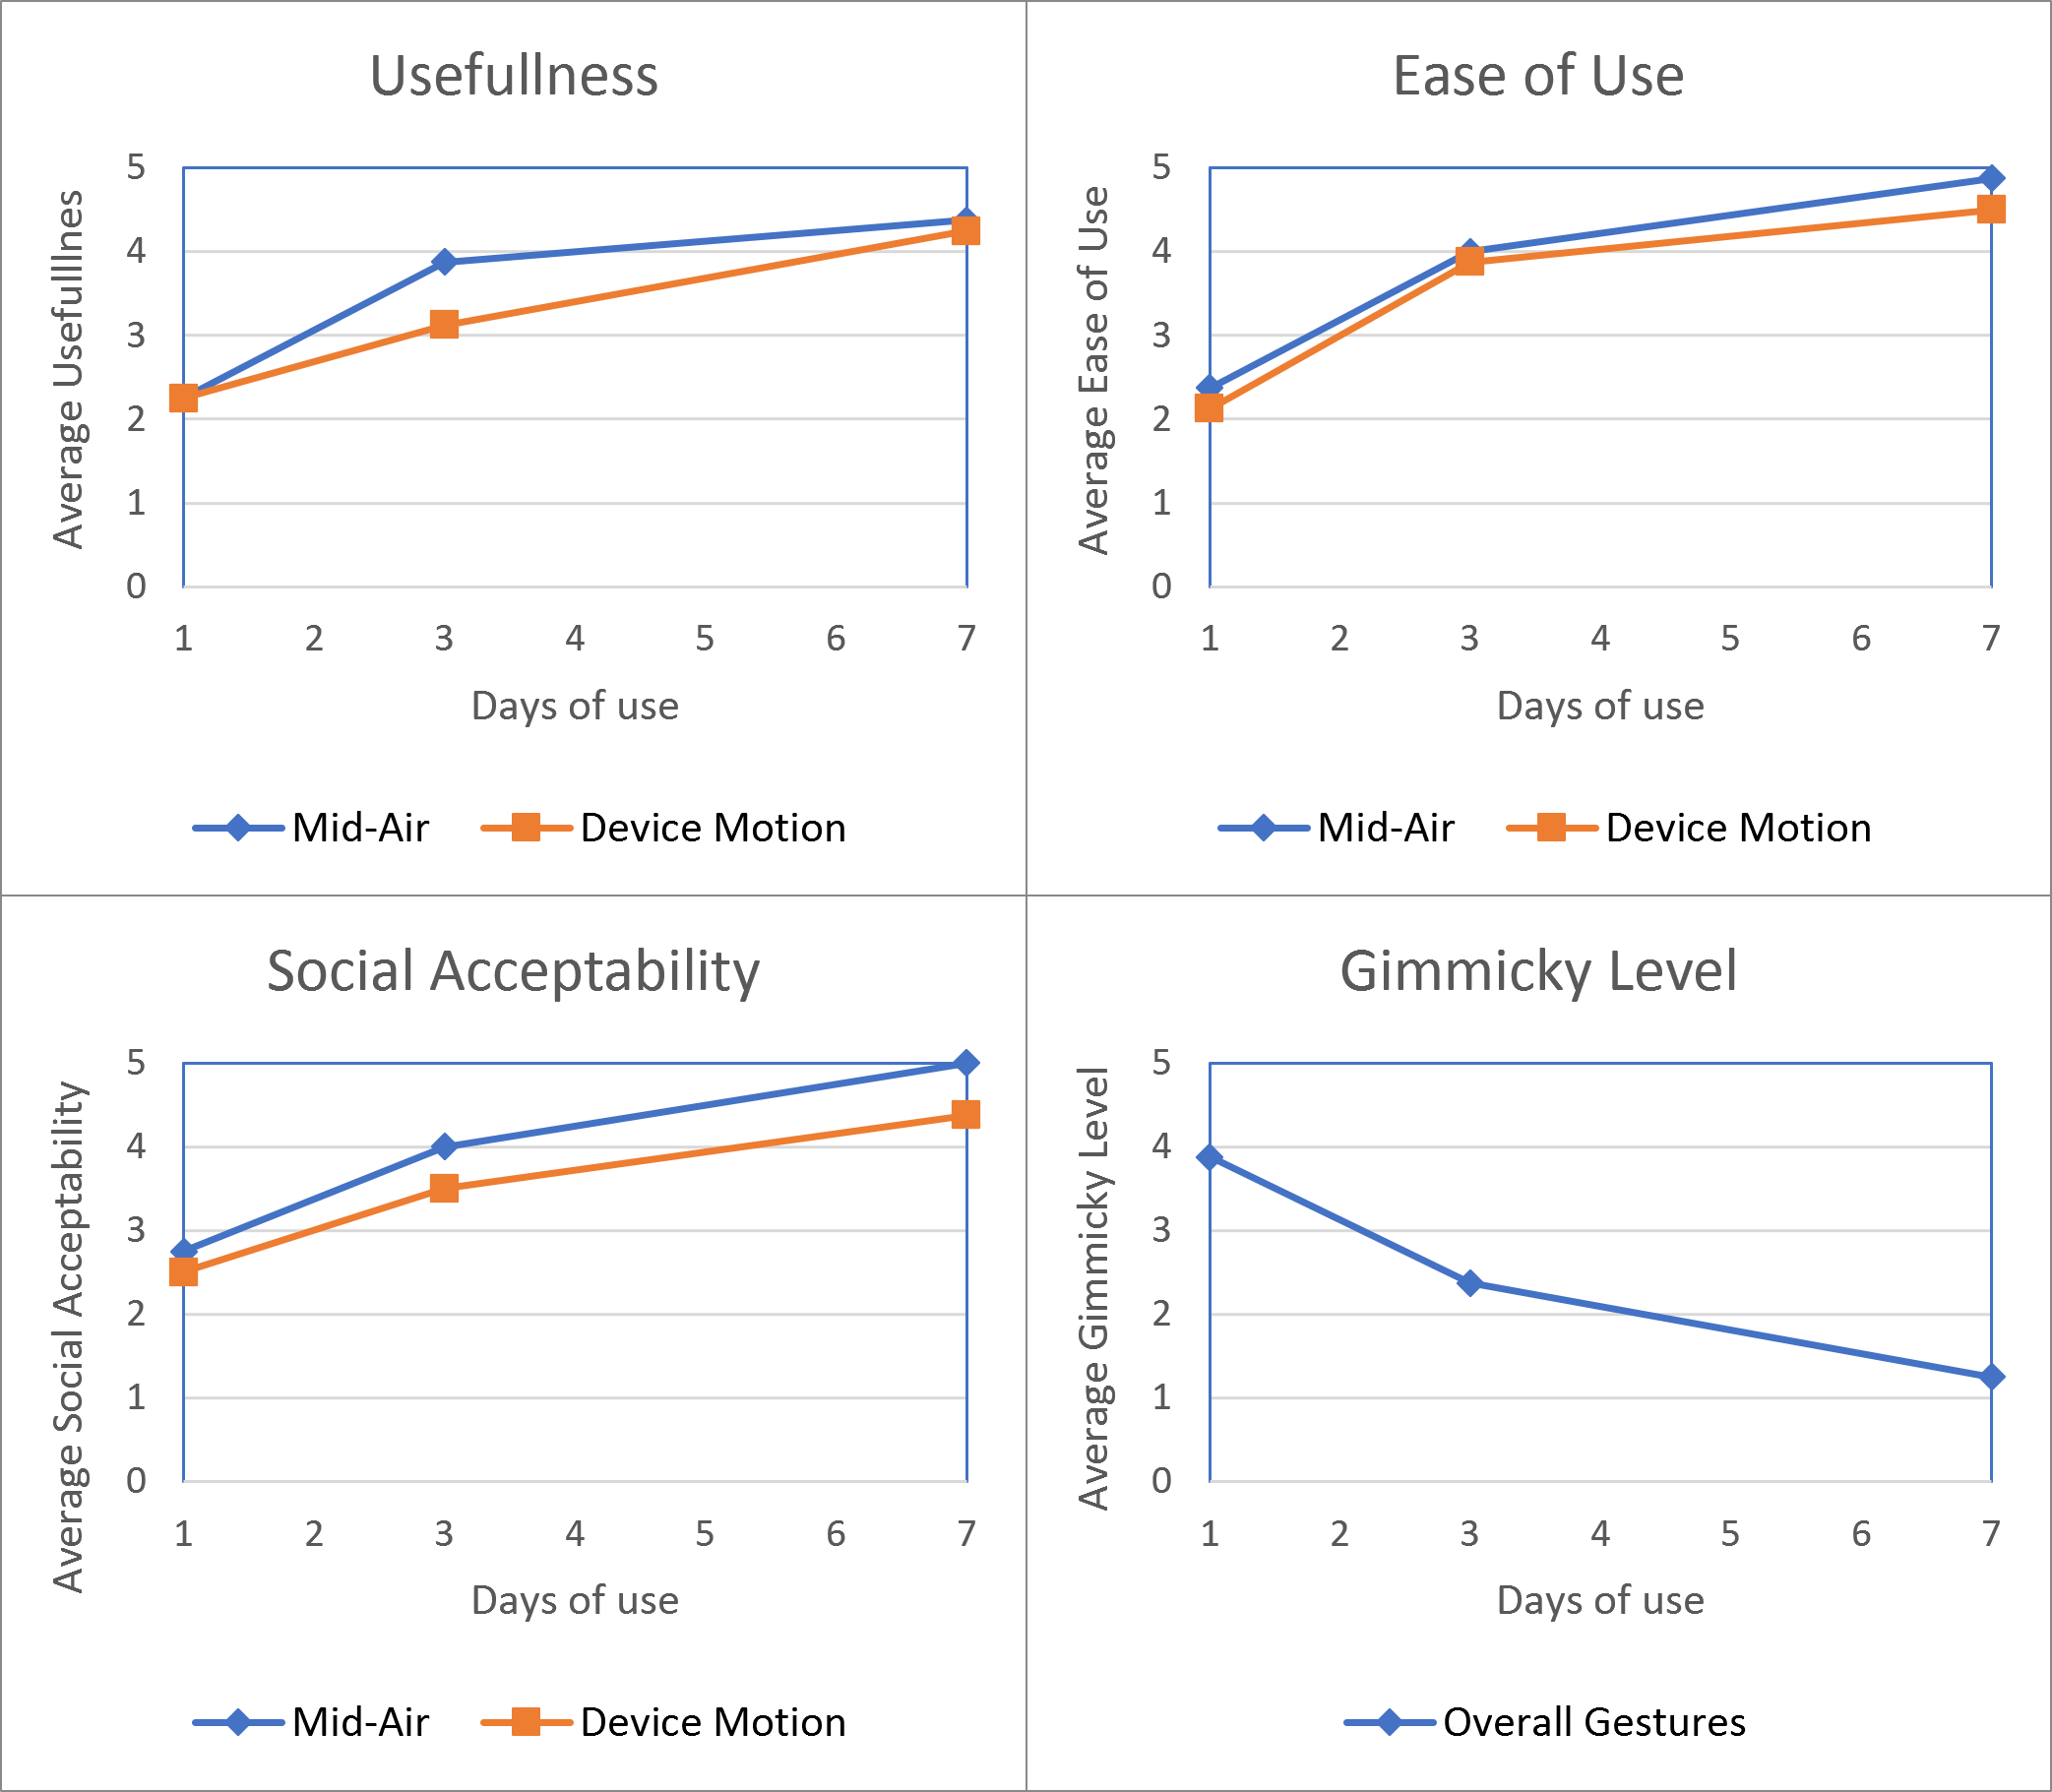
\includegraphics[width=0.8\textwidth]{images/Combined Preceptions.png}
        \caption{Line Graphs showing the average participants' responses for perceived Usefulness, Ease of Use and Social Acceptability for the device motion gestures and mid-air gestures and perceived Gimmicky Level for gestures as a whole.}
        \label{fig:perceptions}
\end{figure}

\subsection{Qualitative Feedback}

After one day of use, Five of the eight participants noted ``I found it fairly hard to get in the way of using the gesture functions'' and those who did not were making the conscious decision to attempt to get in the way of using the gestures and get better at using them. After three days of use, four noted ``I consciously went out my way to try the gesture functions'', two said they ``Tried to get better and more used to using the gesture functions'' and two noted ``I found myself using the gesture functions without thinking about it''. Whereas, after a week of use, 5 of the eight participants strongly agreed that they had started us use the novel interaction techniques without consciously thinking about it and the remaining participants agreeing. All the participants strongly agreed that using the app over the week had made them more open to using these types of interaction in more social situations than they would have before using the app and/or believe that mainstream applications do not currently and could make use of device motion and mid-air gestures.

At the end of the study, 6 of the participants noted that they felt the mid-air gesture was easier than the device motion gesture and all but one participant thought the mid-air gesture was more useful than the device motion gesture.

After a week of use, users provided usage scenarios where either gesture may not be acceptable, user responses of these situations are listed in \autoref{table:Situations}. Six said that they may not use the device motion gesture in a cramped situation where it may result in physical contact with others or intruding in their personal space (e.g. whilst sitting next to them on public transport). One participant noted that they would prefer to not perform exhaustive large movements when with their friends or in a meeting. Only one participant was able to provide an example of when it may be unacceptable to use the mid-air gesture. They stated that it may seem a bit odd in the beginning, but it would become more normal as time passed. Since only one participant was able to provide a response, the majority of participants were confident using the mid-air gesture in any situation. Emphasising their perceived social acceptability of the interaction modality.

\begin{table}[h!]
    \centering
    \begin{tabular}{ | c | m{5cm} | m{5cm} | }
	    \hline
	    Participant & Device Motion Gesture & Mid-Air Gesture\\
	    \hline
        A & When screen is not readable so cant press button & None\\
	    \hline
        B & Possibly not on a cramped train as the may not be space to shake the phone & None\\
	    \hline
	    C & If I'm in bed it might not be reasonable to be shaking my phone & None\\
	    \hline
	    D & When you're listening to music with headphones on in a small enclosed public space, e.g. the subway, the shaking may be annoying to others around you since you're often packed in quite tight. & None\\
	    \hline
	    E & In a meeting or around friends as it's quite a big obvious movement & None\\
	    \hline
	    F & When Shaking would bump into people & None\\
	    \hline
	    G & If you were sitting on public transport and it was very busy and you have people close besides you - could accidentally elbow them & I think at the beginning it would be a bit weird. however, once it was mainstream I doubt there would ever be any reason not to\\
	    \hline
	    H & In crowded places & None\\
	    \hline
    \end{tabular}
    \caption{Situations where participants felt they would be uncomfortable using either gesture type}
    \label{table:Situations}
\end{table}

Users were asked if they could provide any other functions where these types of gesture interactions could be implemented. All participants responded with an example of an existing output with the gesture as an alternative way of controlling it. An example of this was to tilt to the side to remove all notifications. 4 participants providing reasoning for their example that involved the gesture being used in a circumstance when the touch screen method of control required more effort than it normally would complete the task. Following the previous example, using the gesture can take less time and effort than stretching to the top of the screen to remove the notifications using the touchscreen.


\section{Discussion} 

\subsection{Usage Habits}

Initially, the device motion gesture (shake to play a random song) was only used infrequently, less than once per-use of the music player app. This is likely because users would perform this action to start playback, then later switch to other input modalities for changing song (if at all). Its usage frequency generally increased over the course of the week. The mid-air gesture (hover to toggle playback state) was used more frequently than the device motion gesture and its usage increased over the week of the evaluation period. Thus it thought to be due to greater demand for access to this functionality. This indicates that gestures should be designed to control functions that users use more frequently as this may increase the rate at which they will become more used to using them.

\subsection{Perceived Usefulness, Usability and Acceptability}

Perceived usefulness increased over the course of the week. For the mid-air gesture, the largest increase came between Day~1 and Day~3. This is likely because, during this initial period, users had discovered the utility of this function as a more convenient alternative to the touchscreen for quickly toggling playback state. Some participants explained they preferred the mid-air gesture when the effort to use the touchscreen was increased, for example when cooking, to avoid needing to wash your hands first so the screen did not get dirty. In this instance, the cover gesture required no contact, so handwashing was not necessary. When using the touchscreen was more difficult or inconvenient than normal, the contactless gesture was a more appealing option.

As expected, people will come across more useful functions over time, increasing their perceived value. This is indicative that gestures should be considered as an alternative method to functions that are generally controlled by the touchscreen but may have common occurrences where this may be more difficult to use or where additional steps are required. These occurrences have been found to be when the users are moving, and precision touch screen touches cannot be made or where an additional task is being undertaken in parallel to interacting with the device. When the user’s attention is divided, for example cooking or driving using the touchscreen becomes more difficult. As users discover situations where the gesture interaction requires less effort than touch screen input, users recognise this as the gesture being more useful. This reduction in effort required adheres to the social norms on least effort.

Perceptions of how ``gimmicky'' the gestures were changed significantly throughout the study. After one day of use, participants agreed that the gestures available on the application were gimmicky. However, after only one week of using the gestures, all the participants disagreed that they were gimmicky. After becoming more aware of their potential use, participants stopped seeing them as contrived. This suggests users felt that the gestures genuinely benefited the application and were not just available to be eye-catching or a novelty. They believed they fit well in the context of the application and did not lack value. Users found the gestures fitting for general use. It can be assumed that his clear purpose contributed to their good level of perceived social acceptability.

Discovering new uses did not necessarily correspond to the perceived ease of use in the same way that usefulness did. Like with perceived usefulness, ease of use for both gestures increased more rapidly at the beginning of the experiment, levelling off slightly towards the end. Both sets of data are more statistically different between 1 and 3 days of use than between 3 and 7 days of use. This is particularly significant since there was more time between 3 and 7 days of use to become more used to the gestures than there was between 1 and 3 days of use. Participant usage was much higher between 3 and 7 days, yet there was still a larger change in the first three days. This suggests the ease of use of an unfamiliar interaction technique becomes easy to use after as little as three days. This continued to require less effort to use until almost all participants strongly agreed that it took little to no effort to use mid-air gestures. It can be said that the more a person uses a new interaction method, they will become more used to using it and feel as though the desired outcome requires less effort to accomplish a task.

As time passed in the study, data collected showed that there was a strong suggestion that the usefulness of both gesture types increase markedly, and the effort required to use the gestures decreases significantly, particularly in the first 3 days. There is also a significant increase in participants perception of the gesture’s social acceptability between 1 and 3 days and 3 and 7 days of use. Confirming that participants will find the gesture interactions more useful and easier to use over time, and in turn, it will be perceived to be socially acceptable to use in more situations. This is particularly interesting as after even a short period of time of using the application, users’ views on how comfortable they would be using the gestures in an unfamiliar location, or in front of an unfamiliar audience, had noticeably changed positively. These are the factors that many other studies \citep{rico_usable_2010, freeman_rhythmic_2017, ahlstrom_are_2014} suggest are key factors affecting social acceptability. In this case, only a few days of becoming familiar with gestures had completely changed users’ views on using them in these previously thought to be unacceptable circumstances. When designing gestures and other novel interaction techniques, there should be particular considerations for the effort required to complete the task in comparison to what is gained by completing the task. There should be a focus on implementing alternative interactions for when the standard method commonly becomes more difficult due to divided user attention.

Overall, these findings suggest if an interaction technique is easier to use, or if it can be learned easily, then users may start to form a more positive perception of its social acceptability. Adding to this, the more a person uses an application and experiences interactions like gestures, the more likely it is that they will find themselves in situations where the gestures can be more convenient and/or useful than alternative input methods. Following from this, the more frequently a user finds circumstances in which this is the case towards the start of using a novel interaction technique, the more comfortable they will be when in unfamiliar places or with particular people. Results here suggest these changing perceptions can occur in as little as seven days of starting to use features like these.

\subsection{Qualitative Feedback}

All participants agreed that they were using the gestures without thinking about it after the week of use, indicating that there was almost no cognitive load required. This perceived mental invisibility of the gesture again indicates that the user did not have to consciously decide if the outcome of the task was worth the effort required to complete it. The potential for the gesture to be socially unacceptable was not something that crossed the users' minds, confirming that they were perceiving the gestures to be socially acceptable. This then follows that if a user does not have to consider the conservation of energy for completing a task, it is unlikely that they would think about it enough for it to be perceived to be socially unacceptable.

At the end of the study, participants strongly agreed they felt more open to using gestures and believed they could be used more by application and device designers; they were happy to use gestures and were looking to the future and seeing their potential benefits. Their comments suggest they found them useful and the possibility of them being seen to be socially unacceptable had diminished. After only a single week of use, users’ opinions of the Motion Music application's gesture interactions had completely changed: from not being confident or willing to use them around others, to feeling comfortable continuing to use them.

All users provided an example of an existing output with the gesture as an alternative way of controlling it. Half of these responses additionally providing an explanation where the gesture was being used when the touchscreen alternative required an excess of effort to complete. Users would prefer to use and be comfortable using gestures in a wider range of locations and around more people if these details were in mind during creation. This backs up that functions that are often used in situations where it may be more difficult to use the touch screen or where additional steps are required should be considered to have a gesture alternative. 

There was a clear preference for the mid-air gesture. Users felt that this interaction method was easier and more useful than the touchscreen alternative: they could quickly hold their hand above the device with no need for precision. When asked to suggest situations where either type of gesture would be unacceptable, participants found it much easier to identify where device motion gestures would be unacceptable. It was often detailed in these reasons stated in \autoref{table:Situations} that the potential for physical contact would be a key concern. This is counter to what participants expected to be the immediate reason for unacceptability. In the initial survey before use, it was the common theme that effort required was what worried the participants. This indicates that at the forefront of user’s minds is appearing to exceed the social norms of least effort which is then followed by many of the attributes such as location, company and notability detailed by \citet{rico_usable_2010} and \citet{pohl_focused_2013} and other previous work. This was less of an issue with the mid-air gesture. Due to the invisible and concealed nature of the mid-air gesture, which appears more like reaching for the device, participants did not contemplate the potential for physical contact with others.

\subsection{Reflections}

Some findings from this study have implications for the design of new interaction techniques so that user interfaces can be designed to foster more positive perceptions from first use. There was a relationship between social acceptability the perceived effort required to use them, with perceived effort declining with increased exposure to the interactions. Rather than spontaneously waiting for users to discover or start using alternative interactions, apps and user interfaces should encourage more use from the beginning, e.g. training or inviting users to use the interactions. The opportunity to `practice' in a comfortable environment (where social acceptability is less of a concern~\citet{rico_usable_2010}) can help to shape perceptions of effort so that users recognise the utility and convenience of effort-saving interactions~\citet{pohl_focused_2013}. Devices and their features where social acceptability is a concern should  be marketed so the use is not only clear but beneficial to the us

Emphasising the benefits of these as \textit{alternative} interactions for convenience, rather than independent features, in their own right, can help to foster a better impression. Participants here showed reluctance to use motion or mid-air gestures if they were the only way of using an interface. Similarly, participants also indicated a desire for gesture capabilities for \textit{other} functions and apps they already use, not as a novelty but as a convenient alternative that they now recognised the potential benefits of. Another area where gestures may be beneficial is providing an alternative to speech user interfaces in situations where speech could be disruptive or socially unacceptable, like in a library. Helping to shape a positive perception through priming users like this could see more uptake of gesture interactions in smartphones (which have yet to catch on).

Participants also noted the potential for accidentally making physical contact with others when making gesture movements in public spaces. This should consider when designing gestures, in particular, but also for other novel interaction techniques that may require body movement.

%==================================================================================================================================

\chapter{Conclusion}  

\section{Summary}
This project investigated the social acceptability of gesture interaction techniques, focusing in particular on three dimensions: perceived usefulness, perceived effort, and social norms of least effort. Reducing the appearance of `trying too hard' influences peoples' behaviour so this work investigated whether or not this affected human-computer interaction in a similar fashion.

An initial survey was carried out in which respondents were asked about the role of `effort' within social norms and their opinions of the social acceptability of various novel interaction techniques. They were also asked to propose potential gestures that could be used for different tasks. It was found that participants are very aware of the social norms of least effort and the implications it could entail. Participants understood that interactions may often be viewed as socially unacceptable for a variety of reasons. They also indicated wearable interaction and voice assistants could be more unacceptable than gestures in the contexts provided, although were unsure about what types of gestures might actually be used for input.

An evaluation investigated how users’ perceptions of effort, usefulness and social acceptability changed over the course of a week-long study with an interactive music player app for a smartphone. Two gesture controls --- one device motion gesture and one mid-air gesture --- were designed and implemented. An Android music player application was created with these gestures, providing study participants an interface to use these interaction techniques throughout the study period. Users were provided with this application for remote evaluation over the course of a week. Their usage habits, perceptions and opinions of the application and its gestures were recorded through four surveys, spaced out over a week.

The study found that as time passes, participants used the gestures more frequently. Also, over time, perceived usefulness and perceived ease of use increased. Usefulness was found to be greatly enhanced when users were confronted with instances where the touch screen interaction was more difficult or inconvenient (e.g. when handling other items or when needing to interrupt playback while eating). These factors increased quickly over the first three days, levelling off towards the end of the week.

It was apparent that users became more confident in using the gestures in unfamiliar locations and company at a very similar rate in which they felt usefulness and ease of use increased. Findings suggest a link between social acceptability and perceived effort required for interaction: as participants feel like an interaction becomes more effortless, they feel more comfortable using it. Participants were found to hold a positive position for the future of gesture interactions, particularly for mid-air gestures which were unfamiliar to participants prior to this study.


\section{Limitations}
The primary limitation that affected this research was the COVID-19 pandemic and the restrictions it imposed on evaluation. The restrictions and social distancing guidelines meant face-to-face usability studies were not a viable option. An implication of this is that specialised hardware was unsuitable for use (e.g. smart-glasses, interaction sensors like Leap Motion, wearable devices, etc), as these would need to be shared by participants and the evaluator. Instead, remote evaluation was necessary, using devices and capabilities that are widely available (in this instance, via smartphones). This constrained the range of novel interaction techniques that could be assessed, and the most feasible options were motion-based and mid-air gesture controls on a mobile device. Another impact of this is that the sample size in the user study was lower than it may have been in normal circumstances, as arranging remote participation was difficult. Finally, participants typically completed the evaluation in their own homes, a situation where interactions like these are more likely to be seen as socially acceptable~\citet{rico_usable_2010}.

Device motion and mid-air gestures were the main interaction modalities considered in the evaluation. The results and conclusions drawn from the research may not necessarily be true for other novel interaction techniques (e.g. the use of speech); this is a compelling area for future research.


\section{Implications for Interaction Design}
The findings of this work indicated attributes that must be considered when designing gesture interactions. These interactions should be designed with subtlety and `invisibility' in mind, so that users believe others will not perceive them to be ``showing off'', using more than the minimum effort required to complete an interaction task. 

When designing interactions, there should be a focus on their purpose as an alternative means of interaction, rather than a replacement for the touchscreen. These alternatives should be promoted to users, especially novice or unfamiliar users. These provide a convenient alternative, especially in scenarios when touch screen interaction requires more effort to use than normal or where attention is divided between tasks and a more `casual' alternative is desirable~\citet{pohl_focused_2013}.

Interaction techniques should be designed in a way that users will be able to learn how to use them quickly and they should be encouraged to try them out multiple times when new to using a system. This is potentially beneficial as this work showed frequent use and `practice' can shape perceptions of usefulness and social acceptability very rapidly. Users should never be forced to use a novel interaction technique; alternatives should always be provided. This means that a user can decide to use them where they feel comfortable, which might require positive experiences in a familiar environment first. This will allow them to become more familiar with the technique, increasing their confidence in using them in circumstances previously deemed socially unacceptable.


\section{Future Work}
Social acceptability is a compelling topic for new interactive devices and unfamiliar interaction modalities. This work also looked at new dimensions potentially affecting acceptability (i.e., perception of usefulness, perception of perceived effort, perception of `trying too hard'). Further studies should be done with a focus on other types of novel interaction techniques and devices, such as voice assistants and wearable devices, to see how these dimensions are perceived. Following the COVID-19 pandemic, this research could be repeated to ensure a wider sample size and to encourage participants to use the gesture interactions in a variety of locations (to see how this impacts their perceptions of social acceptability over the week of the evaluation). Future developments should consider a study over a longer period than one week, to determine at what point, if at all, the attributes such as ease of use stop increasing. A better understanding of change over time could help identify additional factors that affect the perceived effort needed to use a system, perhaps giving insight into how this can be reduced more rapidly. 

There should be additional research carried out to explore what other attributes can impact how quickly a user can become comfortable using an interaction technique. This should be done with the aim of increasing the rate at which the effort required is reduced. In this study, information on how to complete the gestures was provided to the participants before use and they were made aware of these interactions by the evaluator. Future work could explore alternative means of revealing interactions and teaching users how to use them, without prior knowledge, to see how this impacts their willingness to learn and use them. It should be explored if this can be enhanced by including animations or videos of how they can be used that can be accessed when required. It is thought that nudges could be used to direct users towards using gestures when they have not been used for some time. However, caution must be taken to ensure users do not get annoyed or put off by these. Therefore, further research should be completed in this area -- this is especially timely since commodity smartphones (e.g. the Google Pixel and Samsung Galaxy devices) have seen gestures introduced then subsequently removed, perhaps due to lack of awareness that they exist in the first place.

Further work could also explore in more depth the relationship between perceived usefulness, ease of use and social acceptability. This work has suggested that there is a relation between them as they all changed in similar ways across the study. However, it has not been determined if increased usefulness and ease of use causes a novel interaction technique to be socially acceptable, or if it is that a lack of perceived usefulness and ease of use that causes a novel interaction to be seen as socially unacceptable. These are similar concepts with similar results and participants alluded to their connection in qualitative feedback.

%==================================================================================================================================
%  APPENDICES  
\begin{appendices}

\chapter{Ethics checklist}
Below is the ethics checklist that the study adhered to, to ensure ethical approval.
\begin{figure}[h!]
    \centering
    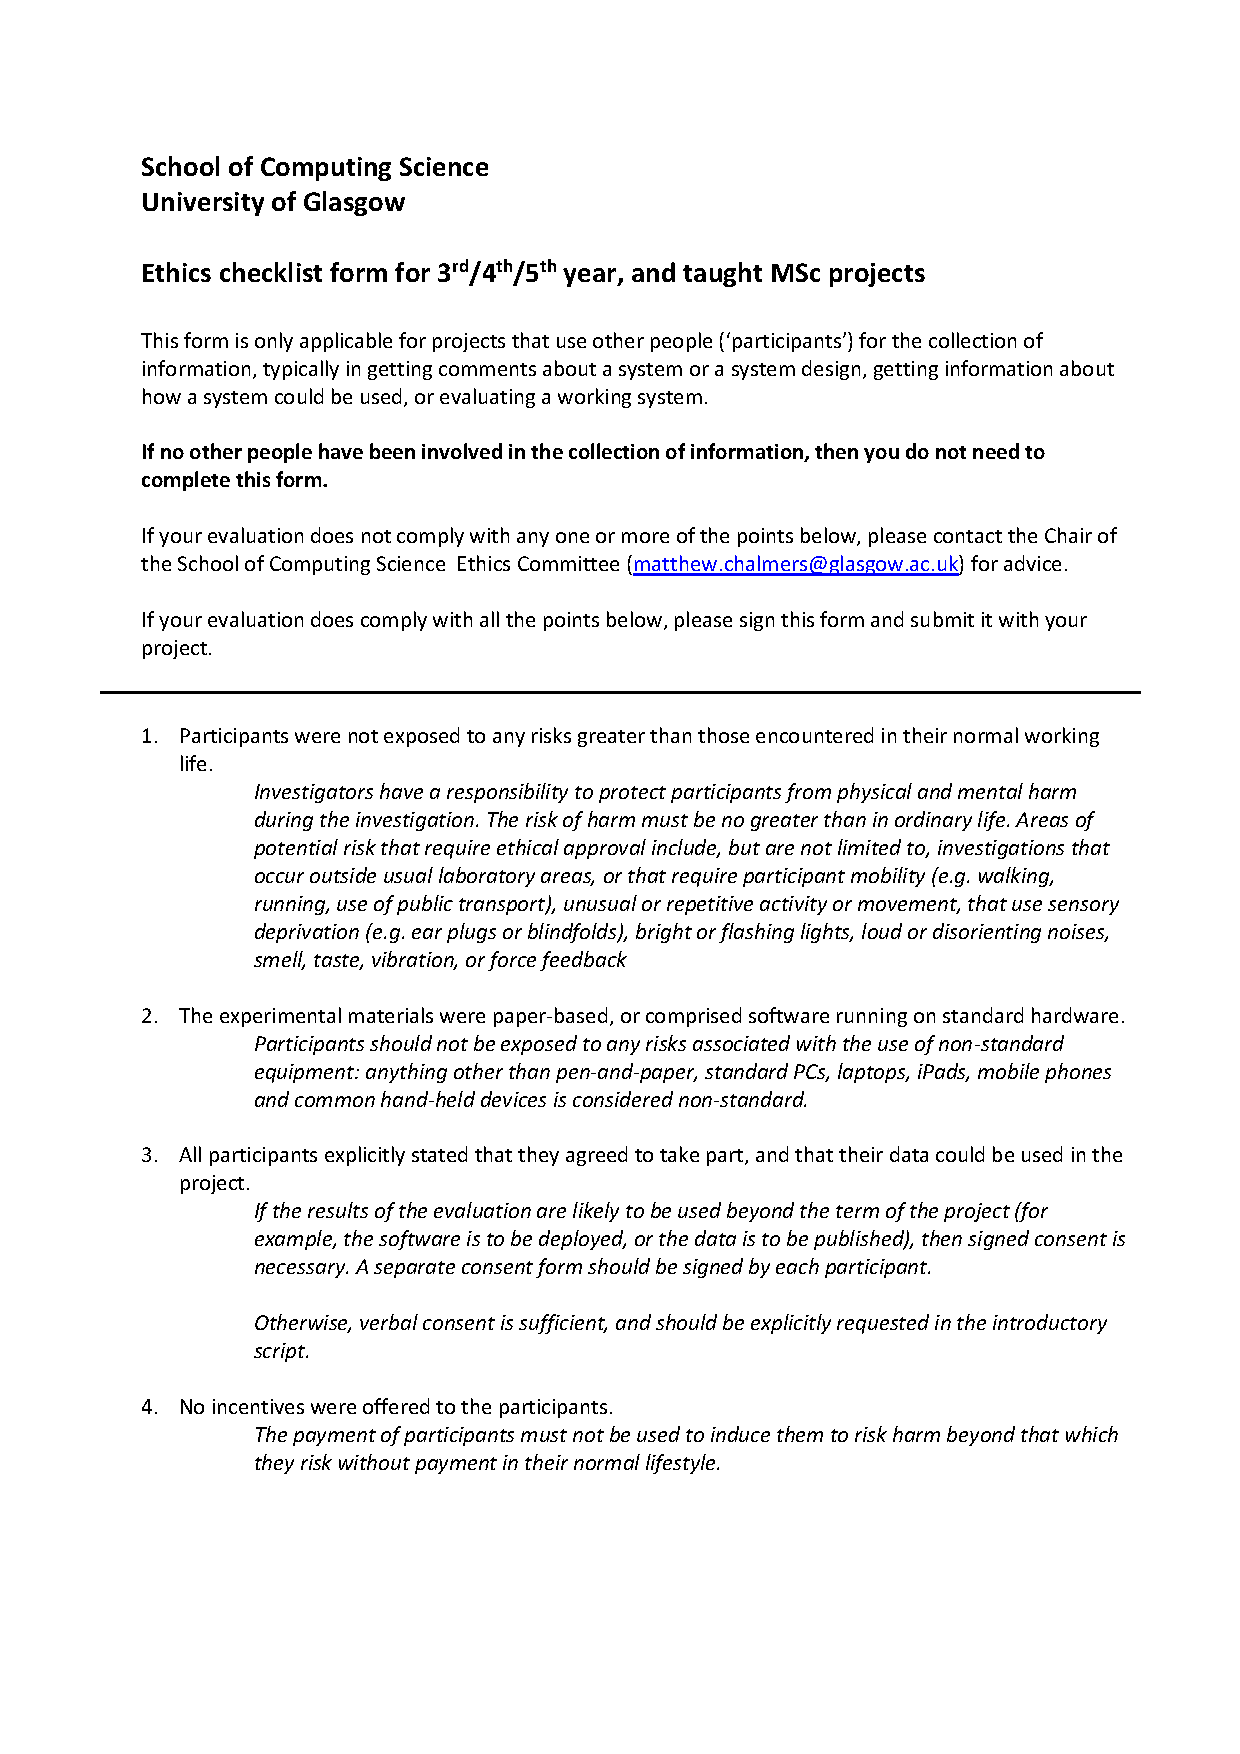
\includegraphics[width=0.85\textwidth]{images/Ethics check-signed1.pdf}
\end{figure}
\begin{figure}[h!]
    \centering
    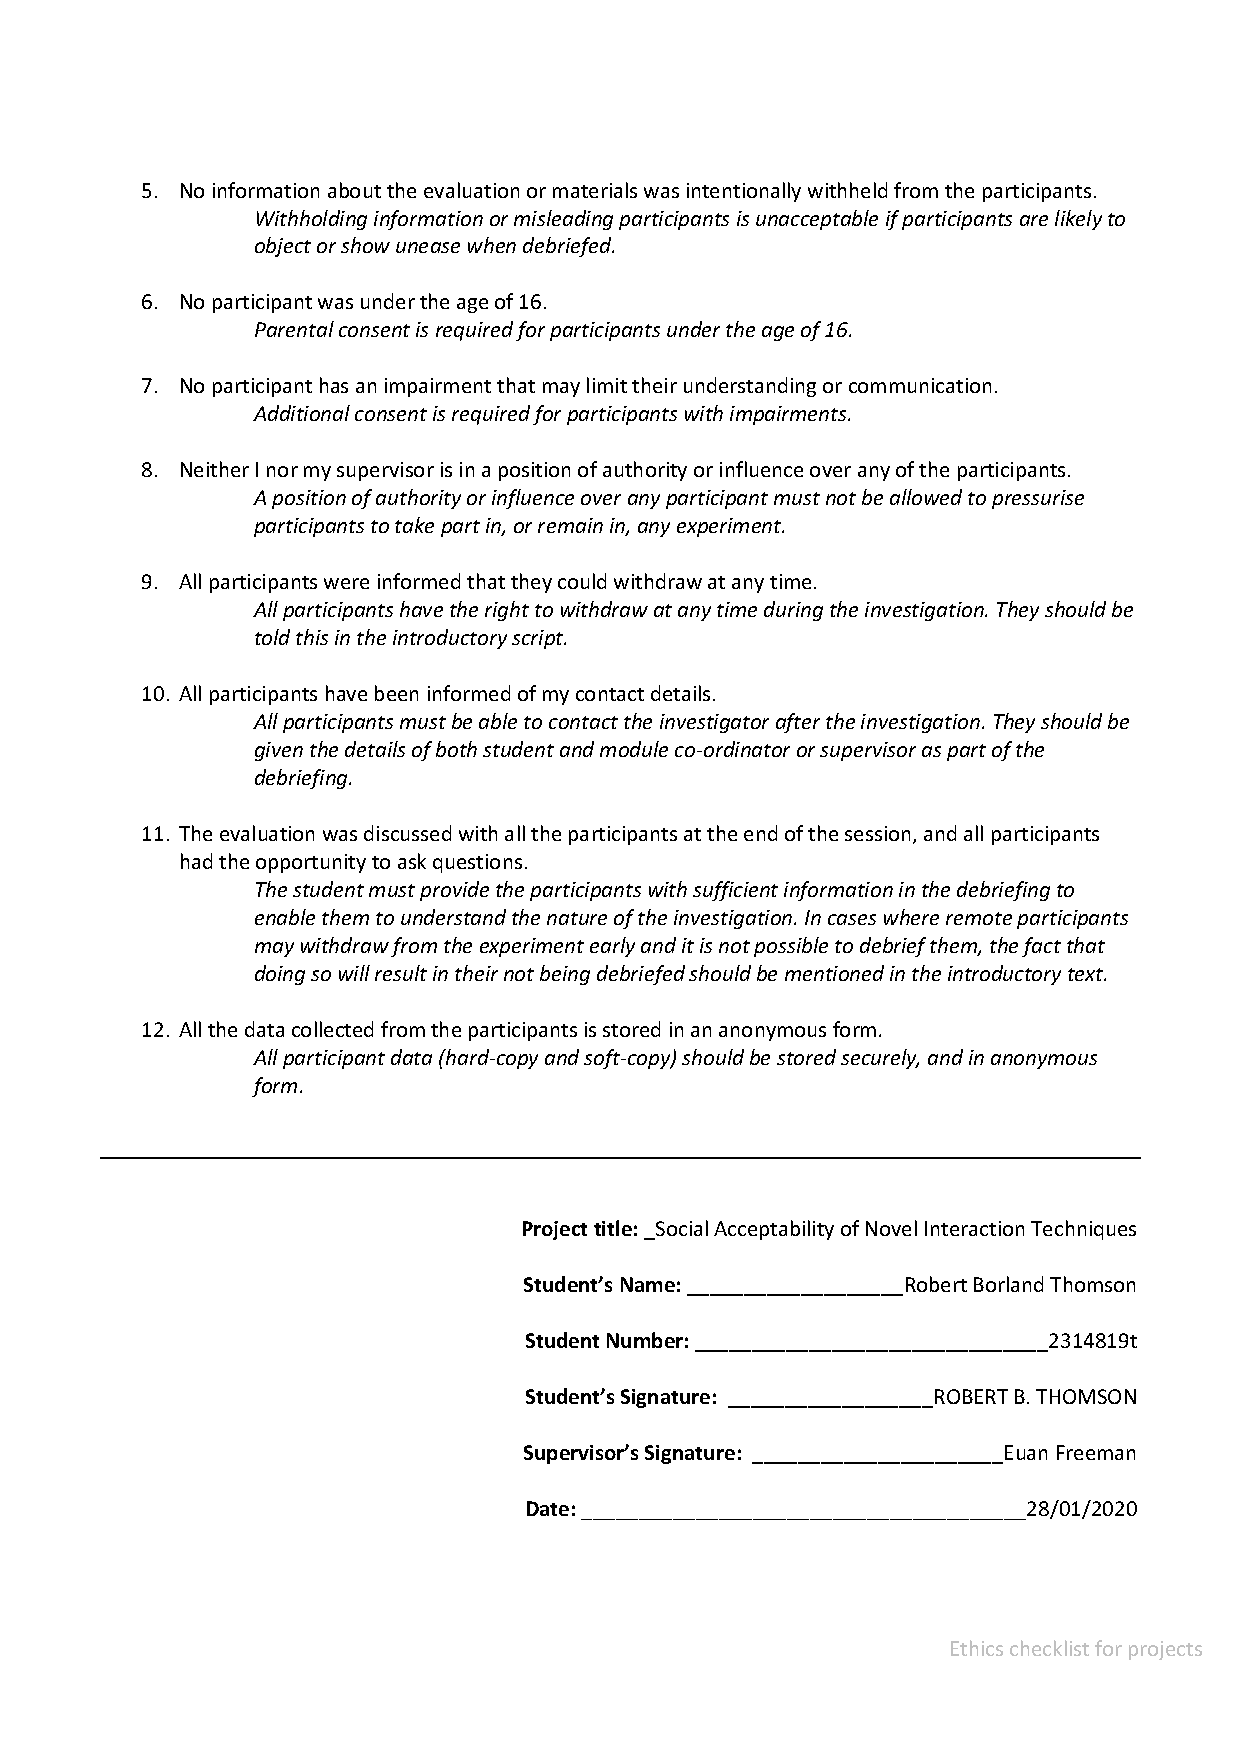
\includegraphics[width=0.9\textwidth]{images/Ethics check-signed2.pdf}
\end{figure}

\chapter{Consent Agreement}
Below is the Consent agreement that all participants of the User Study were asked to complete.
\begin{figure}[h!]
    \centering
    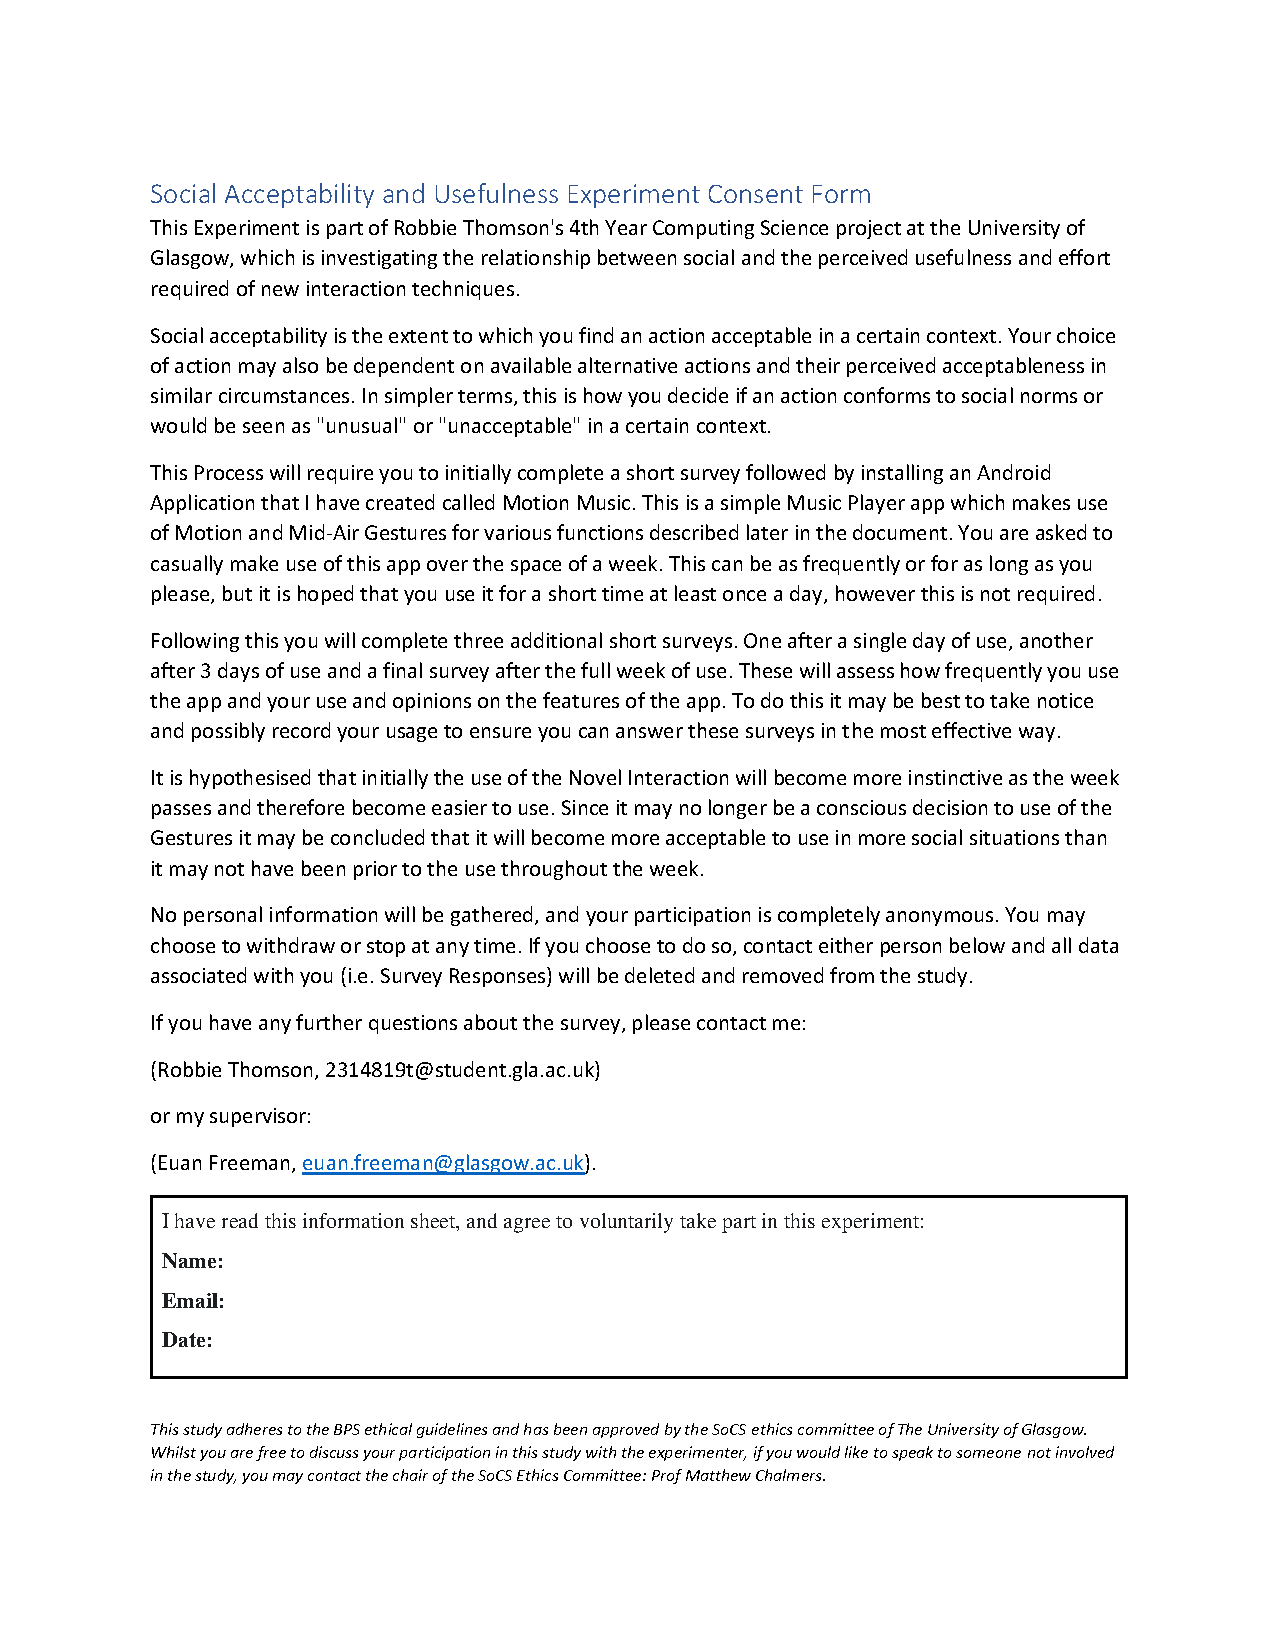
\includegraphics[width=0.9\textwidth]{images/SocialAcceptabilityConsentForm.pdf}
\end{figure}


\chapter{Information Sheet}
Below is the Information Handout supplied to all User Study participants detailing experiment information, installation instructions and Motion Music Usage Details
\begin{figure}[h!]
    \centering
    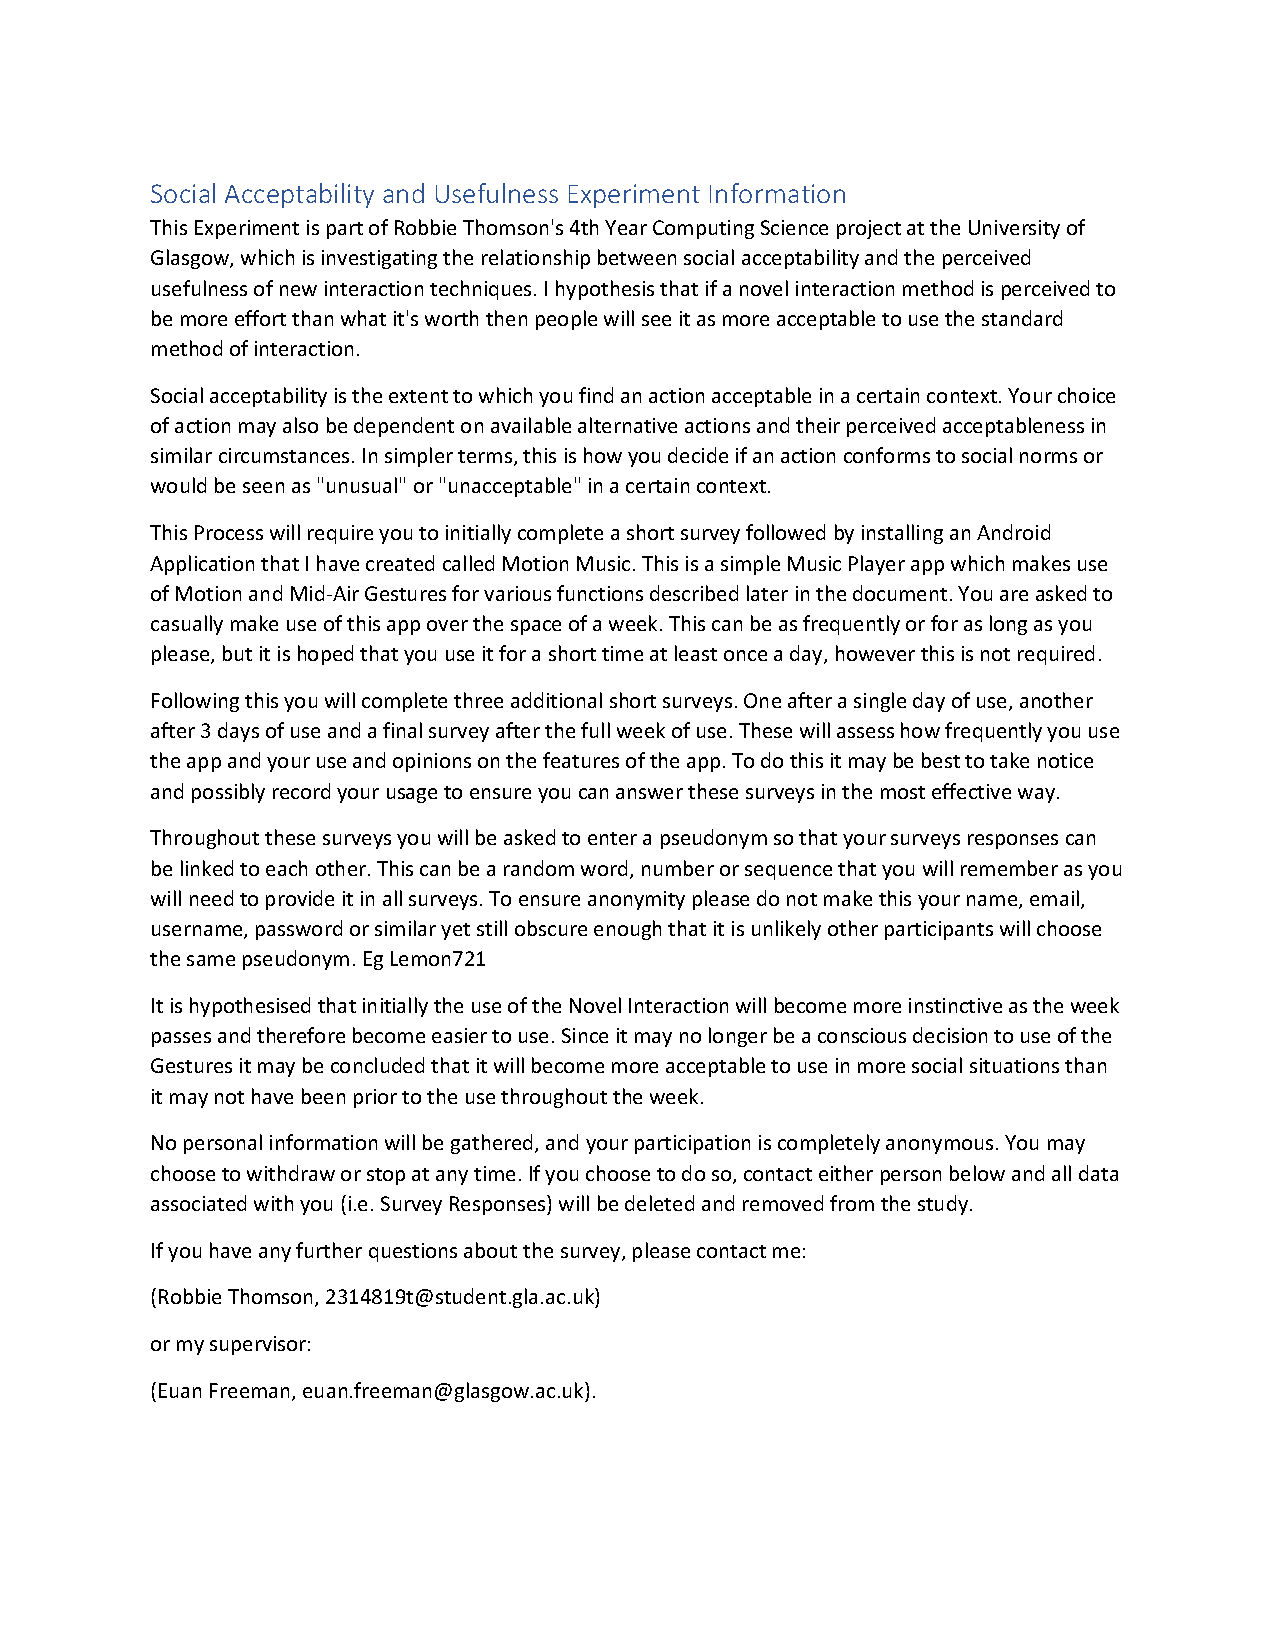
\includegraphics[width=0.9\textwidth]{images/1Info.pdf}
\end{figure}
\begin{figure}[h!]
    \centering
    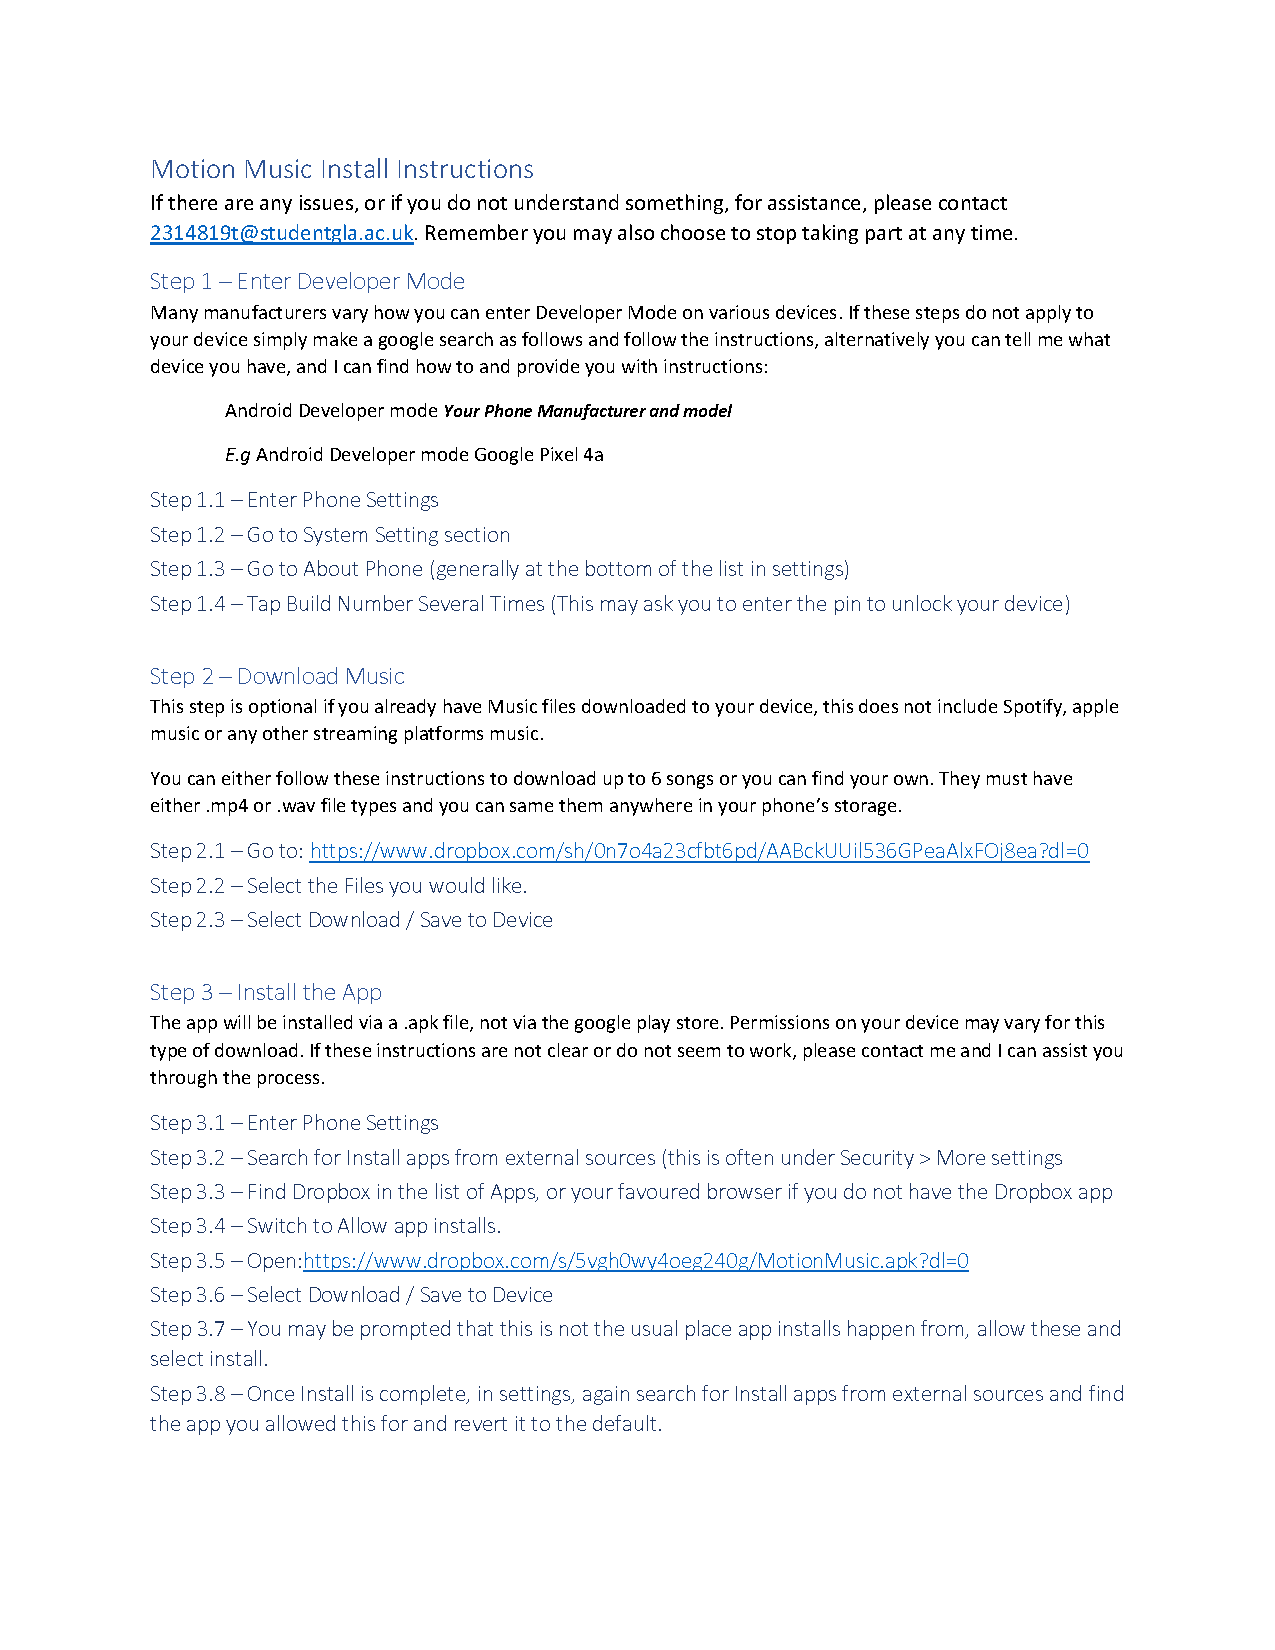
\includegraphics[width=0.9\textwidth]{images/2Info.pdf}
\end{figure}
\begin{figure}[h!]
    \centering
    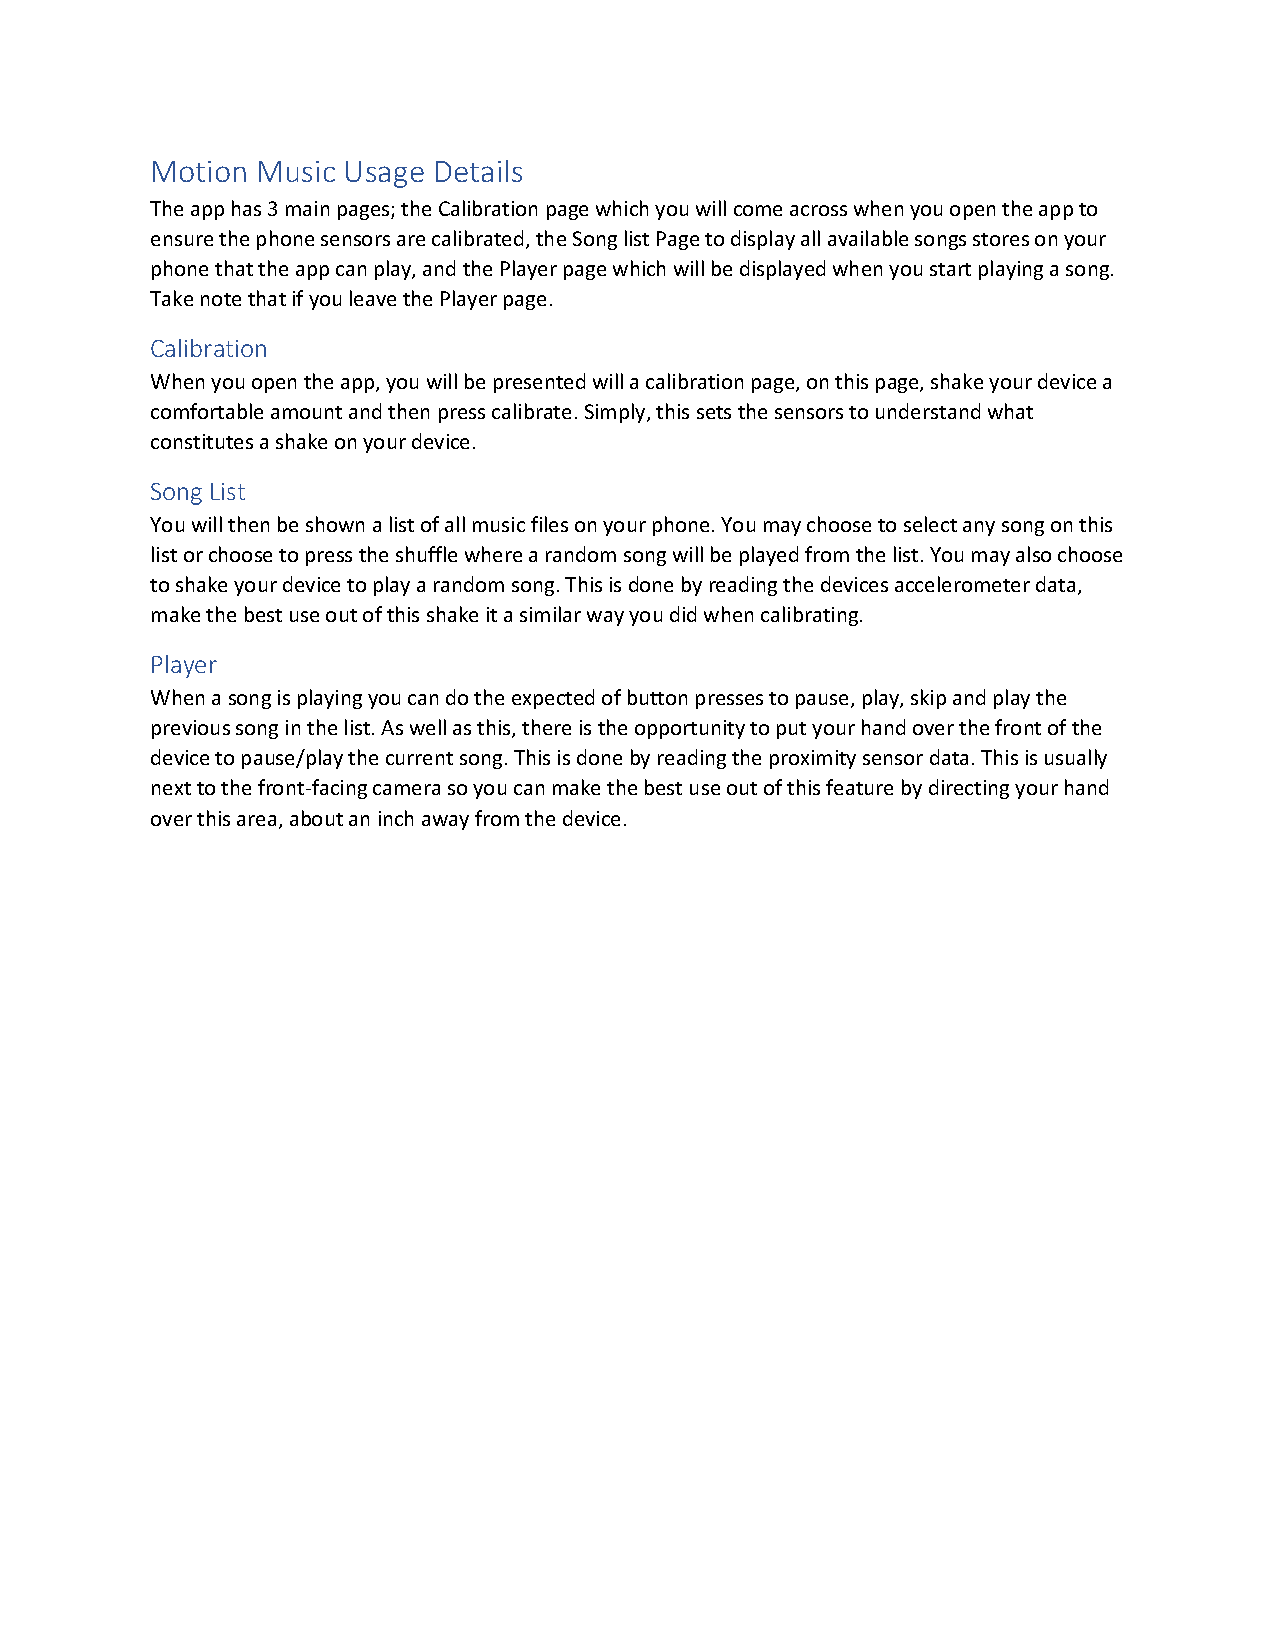
\includegraphics[width=0.9\textwidth]{images/3Info.pdf}
\end{figure}

\chapter{Experiment Debrief}
Below is the Experiment Debrief supplied to all User Study participants
\begin{figure}[h!]
    \centering
    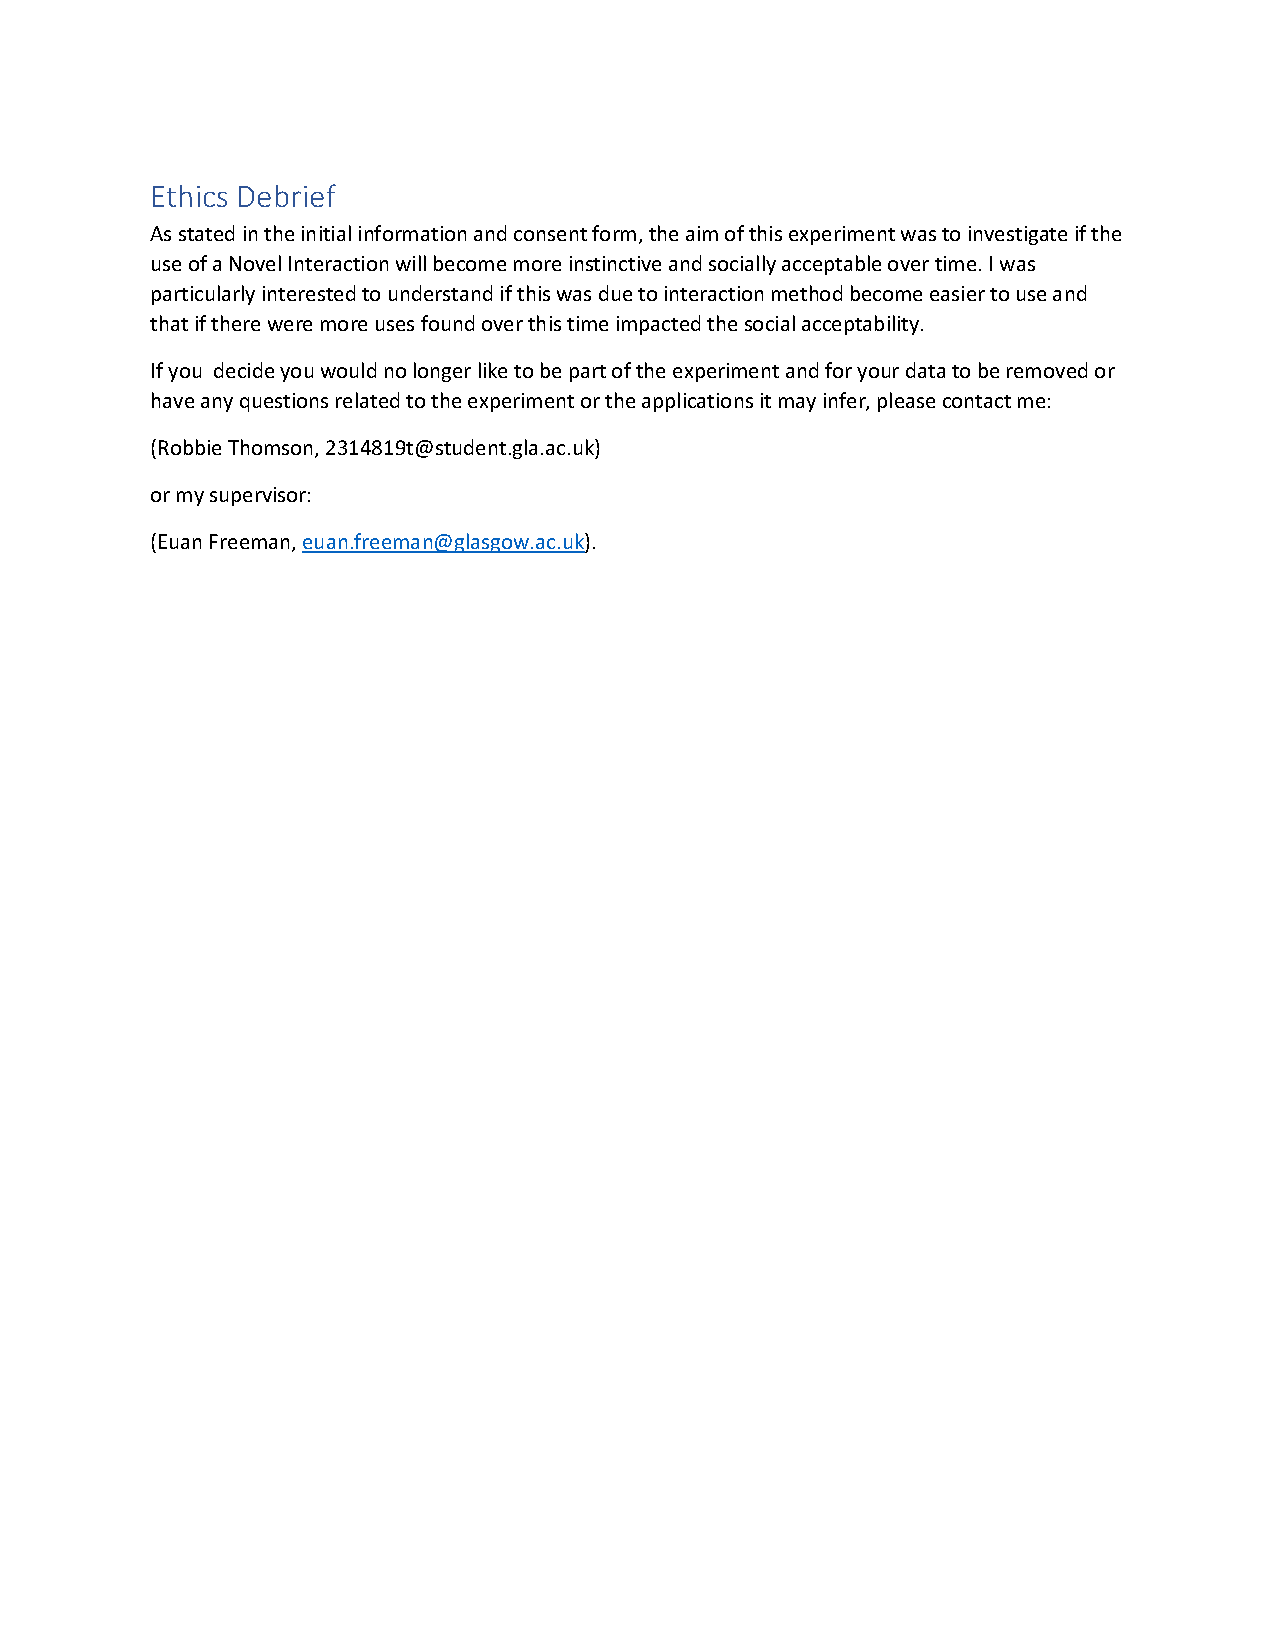
\includegraphics[width=0.9\textwidth]{images/Ethics Debrief.pdf}
\end{figure}


\chapter{Questionnaires}
\label{appendix:questionnaires}
\begin{description}\item Questionnaires used at various stages of the Study\end{description}
\begin{enumerate}
    \item \href{https://docs.google.com/forms/d/1pakX7XYVLeoAOoYjkXVDSh09DWRrcNKFbN93KbzdtMg/prefill}{Link to Questionnaire used in Preliminary Survey Study}
    \item \href{https://docs.google.com/forms/d/1JbD9k1n20KKGAkHvTEXJXE3pGRheN1uez2E0XOwcXZU/prefill}{Link to Questionnaire used in User Study before participant use}
    \item \href{https://docs.google.com/forms/d/1sm2wlPlcC8mvK1OyvnOXUq5_tHZXC1h9BahmidPfutQ/prefill}{Link to Questionnaire used in User Study after one day of participant use}
    \item \href{https://docs.google.com/forms/d/1heEV_uBCCTCK5g-J18M_eL7aD9sfJnWIl7B-Aie7A4c/prefill}{Link to Questionnaire used in User Study after three days of participant use}
    \item \href{https://docs.google.com/forms/d/1NoNhfJRtZiw-utZUCW7sfjN9cYZxTzjtm8tA7g0-hdo/prefill}{Link to Questionnaire used in User Study after seven days of participant use}
\end{enumerate}
    



\chapter{References for music used}
\begin{description}
    \item Art Now by Alex (c) copyright 2011 Licensed under a Creative Commons Attribution (3.0) license. Ft: Snowflake
    \item \url{http://dig.ccmixter.org/files/AlexBeroza/30344}
\item
    \item Dj Rkod - Pulse (George Ellinas Remix) by George\_Ellinas (c) copyright 2008 Licensed under a Creative Commons Attribution (3.0) license.
    \item \url{http://dig.ccmixter.org/files/George_Ellinas/14073 }
\item
    \item There's A Better WAY ! by Loveshadow (c) copyright 2011 Licensed under a Creative Commons Attribution (3.0) license. 
    \item \url{http://dig.ccmixter.org/files/Loveshadow/34402 }
\item
    \item Turning Into Normal (What Once Felt Strange) by SackJo22 (c) copyright 2013 Licensed under a Creative Commons Attribution (3.0) license. Ft: Analog by Nature, Haskel (HE31)
    \item \url{http://dig.ccmixter.org/files/SackJo22/43036}
\end{description}


%\chapter{Tables}
%Extensive tables or figures that are too bulky to fit in the main body of the report, %particularly ones that are repetitive and summarised in the body.


\end{appendices}

%==================================================================================================================================
%   BIBLIOGRAPHY   

\setcounter{chapter}{0}
\bibliographystyle{abbrvnat}

\bibliography{l4proj}

\end{document}
